% Options for packages loaded elsewhere
\PassOptionsToPackage{unicode}{hyperref}
\PassOptionsToPackage{hyphens}{url}
%
\documentclass[
]{book}
\usepackage{amsmath,amssymb}
\usepackage{lmodern}
\usepackage{ifxetex,ifluatex}
\ifnum 0\ifxetex 1\fi\ifluatex 1\fi=0 % if pdftex
  \usepackage[T1]{fontenc}
  \usepackage[utf8]{inputenc}
  \usepackage{textcomp} % provide euro and other symbols
\else % if luatex or xetex
  \usepackage{unicode-math}
  \defaultfontfeatures{Scale=MatchLowercase}
  \defaultfontfeatures[\rmfamily]{Ligatures=TeX,Scale=1}
\fi
% Use upquote if available, for straight quotes in verbatim environments
\IfFileExists{upquote.sty}{\usepackage{upquote}}{}
\IfFileExists{microtype.sty}{% use microtype if available
  \usepackage[]{microtype}
  \UseMicrotypeSet[protrusion]{basicmath} % disable protrusion for tt fonts
}{}
\makeatletter
\@ifundefined{KOMAClassName}{% if non-KOMA class
  \IfFileExists{parskip.sty}{%
    \usepackage{parskip}
  }{% else
    \setlength{\parindent}{0pt}
    \setlength{\parskip}{6pt plus 2pt minus 1pt}}
}{% if KOMA class
  \KOMAoptions{parskip=half}}
\makeatother
\usepackage{xcolor}
\IfFileExists{xurl.sty}{\usepackage{xurl}}{} % add URL line breaks if available
\IfFileExists{bookmark.sty}{\usepackage{bookmark}}{\usepackage{hyperref}}
\hypersetup{
  pdftitle={Climate Change},
  pdfauthor={Dyrehaugen Web Notebook},
  hidelinks,
  pdfcreator={LaTeX via pandoc}}
\urlstyle{same} % disable monospaced font for URLs
\usepackage{longtable,booktabs,array}
\usepackage{calc} % for calculating minipage widths
% Correct order of tables after \paragraph or \subparagraph
\usepackage{etoolbox}
\makeatletter
\patchcmd\longtable{\par}{\if@noskipsec\mbox{}\fi\par}{}{}
\makeatother
% Allow footnotes in longtable head/foot
\IfFileExists{footnotehyper.sty}{\usepackage{footnotehyper}}{\usepackage{footnote}}
\makesavenoteenv{longtable}
\usepackage{graphicx}
\makeatletter
\def\maxwidth{\ifdim\Gin@nat@width>\linewidth\linewidth\else\Gin@nat@width\fi}
\def\maxheight{\ifdim\Gin@nat@height>\textheight\textheight\else\Gin@nat@height\fi}
\makeatother
% Scale images if necessary, so that they will not overflow the page
% margins by default, and it is still possible to overwrite the defaults
% using explicit options in \includegraphics[width, height, ...]{}
\setkeys{Gin}{width=\maxwidth,height=\maxheight,keepaspectratio}
% Set default figure placement to htbp
\makeatletter
\def\fps@figure{htbp}
\makeatother
\setlength{\emergencystretch}{3em} % prevent overfull lines
\providecommand{\tightlist}{%
  \setlength{\itemsep}{0pt}\setlength{\parskip}{0pt}}
\setcounter{secnumdepth}{5}
\usepackage{booktabs}
\usepackage{amsthm}
\makeatletter
\def\thm@space@setup{%
  \thm@preskip=8pt plus 2pt minus 4pt
  \thm@postskip=\thm@preskip
}
\makeatother

\renewcommand\chaptername{}
\ifluatex
  \usepackage{selnolig}  % disable illegal ligatures
\fi
\usepackage[]{natbib}
\bibliographystyle{apalike}

\title{Climate Change}
\author{Dyrehaugen Web Notebook}
\date{2021-04-26}

\begin{document}
\maketitle

{
\setcounter{tocdepth}{1}
\tableofcontents
}
\hypertarget{climate-change}{%
\chapter{Climate Change}\label{climate-change}}

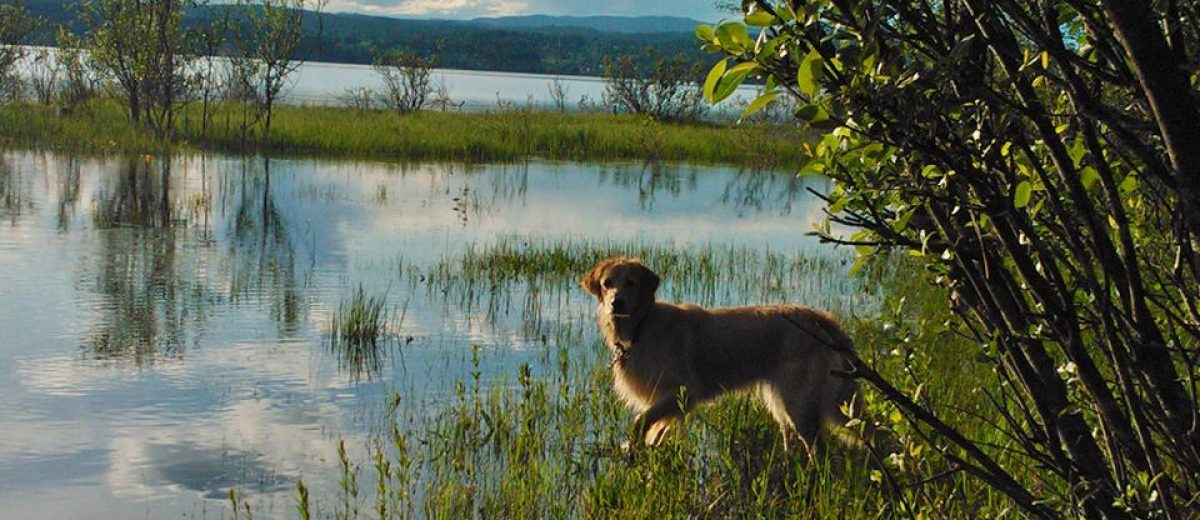
\includegraphics{fig/zelda.jpg}

\hypertarget{neo-liberal-climate-change}{%
\section{Neo-liberal Climate Change}\label{neo-liberal-climate-change}}

The neoliberal solution to climate change is to hope
that somehow it will become profitable to save the planet.
This will not work.
(\citet{ExistentialComics})

\hypertarget{part-climate-models}{%
\part{Climate Models}\label{part-climate-models}}

\hypertarget{climate-models}{%
\chapter{Climate Models}\label{climate-models}}

Overview text on selected Climate Models

\hypertarget{dice-climate-model}{%
\section{DICE Climate Model}\label{dice-climate-model}}

Independent of the
normative assumptions of inequality aversion and time preferences,
the Paris agreement constitutes the economically optimal policy pathway
for the century.
Authors claim they show this by incorporating a
damage-cost curve reproducing
the observed relation between temperature
and economic growth into the integrated assessment model DICE.

\href{https://www.nature.com/articles/s41467-019-13961-1}{Glanemann (2021) DICE Paris CBA}
\href{pdf/Glanemann_2021_DICE_Paris_CBA.pdf}{(pdf)}

\hypertarget{the-failure-of-dice-economics}{%
\subsection{The failure of Dice Economics}\label{the-failure-of-dice-economics}}

If there is one climate economist who is respected above all others, it's William Nordhaus of Yale, who won the Econ Nobel in 2018 ``for integrating climate change into long-run macroeconomic analysis.'' The prize specifically cited Nordhaus' creation of an ``integrated assessment model'' for analyzing the costs of climate change. The most famous of these is the DICE Model, used by the Environmental Protection Agency.

But the DICE Model, or at least the version we've been using for years, is obviously bananas.

\href{https://noahpinion.substack.com/p/why-has-climate-economics-failed}{Noah Smith}

For other economists look here

\href{https://twitter.com/CatieHausman/status/1381999336423362568}{Catie Hausman Twitter Thread}

\hypertarget{ez-climate-model}{%
\section{EZ-Climate Model}\label{ez-climate-model}}

Some text on EZClimate

\hypertarget{fair-climate-model}{%
\section{FAIR Climate Model}\label{fair-climate-model}}

The FAIR model satisfies all
criteria set by the NAS for use in an SCC calculation. 22 Importantly, this model
generates projections of future warming that are consistent with comprehensive, state-
of-the-art models and it can be used to accurately characterize current best
understanding of the uncertainty regarding the impact that an additional ton of CO 2
has on global mean surface temperature (GMST). Finally, FAIR is easily implemented
and transparently documented, 23 and is already being used in updates of the SCC. 24

A key limitation of FAIR and other simple climate models is that they do not represent
the change in global mean sea level rise (GMSL) due to a marginal change in emissions.

\href{Greenstone_2021_Updating_SCC.pdf}{Carleton Greenstone (2021) Updating SCC (pdf)}

\href{https://fair.readthedocs.io/en/latest/}{FAIR}

\hypertarget{global-calculator}{%
\section{Global Calculator}\label{global-calculator}}

Used by Kuhnhenn - STS - Heinrch Böll Stiftung

\href{http://www.globalcalculator.org/}{GlobalCalculator}

\href{http://tool.globalcalculator.org/globcalc.html?levers=22rfoe2e\%2013be1111c2c2c1n31hfjdcef222hp233f211111fn2211111111/dashboard/en}{Global Calculator Tool}

\hypertarget{monash-climate-model}{%
\section{Monash Climate Model}\label{monash-climate-model}}

Some text on Monash Model

\hypertarget{noresm}{%
\section{NorESM}\label{noresm}}

\textbf{Norwegian Earth System Model}

\emph{About}

A climate model solves mathematically formulated natural laws on a three-dimensional grid. The climate model divides the soil system into components (atmosphere, sea, sea ice, land with vegetation, etc.) that interact through transmission of energy, motion and moisture. When the climate model also includes advanced interactive atmosphere chemistry and biogeochemical cycles (such as the carbon cycle), it is called an earth system model.

The Norwegian Earth System Model NorESM has been developed since 2007 and has been an important tool for Norwegian climate researchers in the study of the past, present and future climate. NorESM has also contributed to climate simulation that has been used in research assessed in the IPCC's fifth main report.

\emph{INES}

The project Infrastructure for Norwegian Earth System Modeling (INES) will support the further development of NorESM and help Norwegian scientists also gain access to a cutting-edge earth system model in the years to come. Technical support will be provided for the use of a more refined grid, the ability to respond to climate change up to 10 years in advance, the inclusion of new processes at high latitudes and the ability of long-term projection of sea level.
Climate simulations with NorESM are made on some of the most powerful supercomputers in Norway, and INES will help these exotic computers to be exploited in the best possible way and that the large data sets produced are efficiently stored and used. The project will ensure that researchers can efficiently use the model tool, analyze results and make the results available.

\hypertarget{ccsm4}{%
\subsection{CCSM4}\label{ccsm4}}

\emph{UCAR NCAR}

The University Corporation for Atmospheric Research (UCAR) is a
US nonprofit consortium of more than 100 colleges and universities providing
research and training in the atmospheric and related sciences.
UCAR manages the National Center for Atmospheric Research (NCAR) and
provides additional services to strengthen and support research and education
through its community programs.
Its headquarters, in Boulder, Colorado, include NCAR's Mesa Laboratory. (Wikipedia)

\emph{CCSM}

The Community Climate System Model (CCSM) is a
coupled climate model for simulating Earth's climate system.
CCSM consists of five geophysical models:
atmosphere (atm), sea-ice (ice), land (lnd), ocean (ocn), and land-ice (glc),
plus a coupler (cpl) that coordinates the models and passes information between them.
Each model may have ``active,'' ``data,'' ``dead,'' or ``stub'' component version allowing
for a variety of ``plug and play'' combinations.

During the course of a CCSM run, the model components integrate forward in time, periodically stopping to exchange information with the coupler. The coupler meanwhile receives fields from the component models, computes, maps, and merges this information, then sends the fields back to the component models. The coupler brokers this sequence of communication interchanges and manages the overall time progression of the coupled system. A CCSM component set is comprised of six components: one component from each model (atm, lnd, ocn, ice, and glc) plus the coupler. Model components are written primarily in Fortran 90.

\href{https://www.cesm.ucar.edu/models/ccsm4.0/ccsm_doc/x42.html\#ccsm_machines}{ccsm4}

\emph{CESM}

The Community Earth System Model (CESM) is a fully-coupled, global climate model that provides state-of-the-art computer simulations of the Earth's past, present, and future climate states.

CESM2 is the most current release and contains support for CMIP6 experiment configurations.

\href{https://www.cesm.ucar.edu/models/}{cesm models}

\emph{Simpler Models}

As part of CESM2.0, several dynamical core and aquaplanet configurations have been made available.

\href{https://www.cesm.ucar.edu/models/simpler-models/}{Simpler Models}

\hypertarget{noresm-features}{%
\subsection{NorESM Features}\label{noresm-features}}

Despite the nationally coordinated effort, Norway has
insufficient expertise and manpower to develop, test, verify
and maintain a complete earth system model. For this reason,
NorESM is based on the Community Climate System Model version 4,
CCSM4, operated at the National Center for
Atmospheric Research on behalf of the Community Climate
System Model (CCSM)/Community Earth System Model
(CESM) project of the University Corporation for
Atmospheric Research.

NorESM is, however, more than a model
``dialect'' of CCSM4. Notably, NorESM differs from CCSM4
in the following aspects: NorESM utilises an isopycnic
coordinate ocean general circulation model developed in
Bergen during the last decade originating from the Miami Isopycnic Coordinate
Ocean Model (MICOM). The atmospheric module is modified with
chemistry--aerosol--cloud--radiation interaction schemes developed for the Oslo
version of the Community Atmosphere Model (CAM4-Oslo).
Finally, the HAMburg Ocean Carbon Cycle (HAMOCC) model developed at the Max Planck
Institute for Meteorology, Hamburg, adapted to an isopycnic ocean
model framework, constitutes the core of
the biogeochemical ocean module in NorESM.
In this way NorESM adds to the much desired climate model diversity,
and thus to the hierarchy of models participating in phase
5 of the Climate Model Intercomparison Project (CMIP5).
In this and in an accompanying paper (Iversen et al., 2013), NorESM without
biogeochemical cycling is presented.
The reader is referred to Assmann et al.~(2010) and Tjiputra et al.~(2013)
for a description of the biogeochemical ocean component and carbon
cycle version of NorESM, respectively.

There are several overarching objectives underlying the
development of NorESM. Western Scandinavia and the surrounding
seas are located in the midst of the largest surface
temperature anomaly on earth governed
by anomalously large oceanic and atmospheric heat
transports.
Small changes to these transports may result in large and abrupt changes in the local climate.
To better understand the variability and stability of the climate system,
detailed studies of the formation, propagation
and decay of thermal and (oceanic) fresh water anomalies are required.

NorESM is, as mentioned above, largely based on CCSM4.
The main differences are the isopycnic coordinate ocean
module in NorESM and that CAM4-Oslo substitutes CAM4
as the atmosphere module. The sea ice and land models in
NorESM are basically the same as in CCSM4 and the Com-
munity Earth System Model version 1 (CESM1), except that
deposited soot and mineral dust aerosols on snow and sea ice
are based on the aerosol calculations in CAM4-Oslo.

\hypertarget{noresm-aerosol-interactions}{%
\subsubsection{NorESM Aerosol Interactions}\label{noresm-aerosol-interactions}}

The aerosol module is extended from earlier versions that
have been published, and includes life-cycling of sea salt,
mineral dust, particulate sulphate, black carbon, and primary
and secondary organics. The impacts of most of the numer-
ous changes since previous versions are thoroughly explored
by sensitivity experiments. The most important changes are:
modified prognostic sea salt emissions; updated treatment
of precipitation scavenging and gravitational settling; inclu-
sion of biogenic primary organics and methane sulphonic
acid (MSA) from oceans; almost doubled production of land-
based biogenic secondary organic aerosols (SOA); and in-
creased ratio of organic matter to organic carbon (OM/OC)
for biomass burning aerosols from 1.4 to 2.6.
Compared with in situ measurements and remotely sensed
data, the new treatments of sea salt and dust aerosols
give smaller biases in near-surface mass concentrations and
aerosol optical depth than in the earlier model version. The
model biases for mass concentrations are approximately un-
changed for sulphate and BC. The enhanced levels of mod-
led OM yield improved overall statistics, even though OM
is still underestimated in Europe and overestimated in North
America.
The global anthropogenic aerosol direct radiative forc-
ing (DRF) at the top of the atmosphere has changed from
a small positive value to −0.08 W m −2 in CAM4-Oslo. The
sensitivity tests suggest that this change can be attributed to
the new treatment of biomass burning aerosols and gravita-
tional settling. Although it has not been a goal in this study,
the new DRF estimate is closer both to the median model
estimate from the AeroCom intercomparison and the best es-
timate in IPCC AR4. Estimated DRF at the ground surface
has increased by ca. 60 \%, to −1.89 W m −2

The increased abundance of natural OM and the introduc-
tion of a cloud droplet spectral dispersion formulation are the
most important contributions to a considerably decreased es-
timate of the indirect radiative forcing (IndRF). The IndRF
is also found to be sensitive to assumptions about the coat-
ing of insoluble aerosols by sulphate and OM. The IndRF of
−1.2 W m −2 , which is closer to the IPCC AR4 estimates than
the previous estimate of −1.9 W m −2 , has thus been obtained
without imposing unrealistic artificial lower bounds on cloud
droplet number concentrations.

\href{https://www.noresm.org/}{NorESM}

\href{https://gmd.copernicus.org/articles/6/687/2013/}{Bentsen (2013) NorESM - Part 1}
\href{pdf/Bentsen_2013_NorESM_1.pdf}{(pdf)}

\href{https://gmd.copernicus.org/articles/6/389/2013/}{Iversen (2013) NorESM - Part 2}
\href{pdf/Iversen_2013_NorESM_2.pdf}{(pdf)}

\href{https://gmd.copernicus.org/articles/3/143/2010/}{Assmann (2010) Biogeochemical Ocean Component - Isopycnic}
\href{pdf/Assmann_2010_Isopycnic_Ocean_Carbon_Cycle_Model.pdf}{(pdf)}

\href{https://gmd.copernicus.org/articles/3/123/2010/}{Tjiputra (2010) Carbon Cycle Component}
\href{pdf/Tjiputra_2010_Climate_Cycle_Feedbacks.pdf}{(pdf)}

\href{https://gmd.copernicus.org/articles/6/207/2013/}{Kirkevaag (2013) Aerosol-Climate Interactions}
\href{pdf/Kirkevaag_2013_Aerosol_NorESM.pdf}{(pdf)}

\href{https://www.cesm.ucar.edu/}{Community Earth System Model CESM}

\hypertarget{goal-index}{%
\section{Goal Index}\label{goal-index}}

In economic modelling choice of goal index (utility) function matters.
Daniel 2018\footnote{See Links to references} presents this figure:

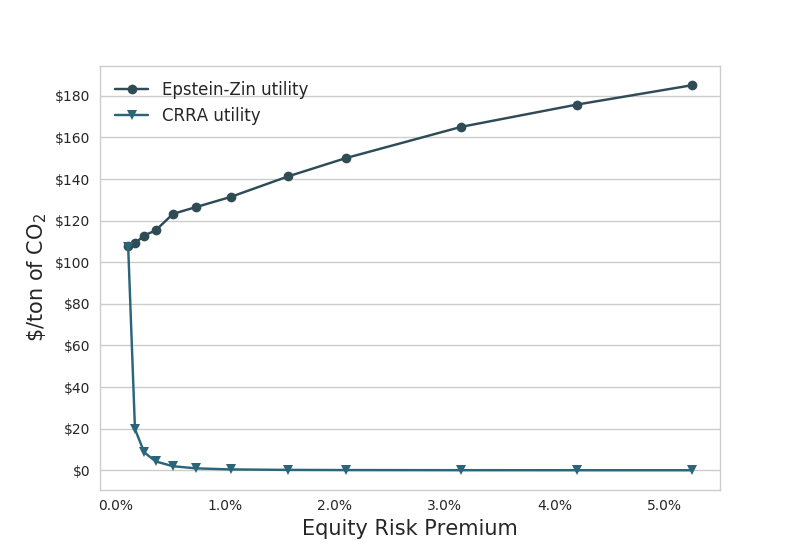
\includegraphics{fig/fig_EZvsCRRA_daniel2018fig1.png}

Fig. Optimal CO2-prices with increasing risk aversion for EZ vs CRRA utility specification. (From Daniel 2018)

As one of the co-authors explain: `We where not able to get the Social
Cost of Carbon (SCC) under \$120'.
That is for `reasonable risk aversion', using EZ-utilities.
The `standard' specification - with CRRA - utilities ends up with SCC
of \$20 or below.

\[V_1 = A [\tilde{C\_t}, \mu_t(V\_{t+1})]\]

Specification of the Goal Index function may seem a trivial technical issue -
no so!
There exists a broad professional litterature and profound discussions on
this matter -
which might de difficult to dis-entangle.

Let us begin with Frank Ramsey's growth model from 1928, commonly known
as the Ramsey-Cass-Koopmans model.

\(F(K,L)\) is an aggregate production function with factors \(K\) (Capital) and
\(L\) (Labour).

\hypertarget{model-drift}{%
\section{Model Drift}\label{model-drift}}

\emph{Abstract Sausen}

A method is proposed for removing the
drift of coupled atmosphere-ocean models, which
in the past has often hindered the application of
coupled models in climate response and sensitivity experiments.
The ocean-atmosphere flux fields
exhibit inconsistencies when evaluated separately
for the individual sub-systems in independent,
uncoupled mode equilibrium climate computations.
In order to balance these inconsistencies a
constant ocean-atmosphere flux correction field is
introduced in the boundary conditions coupling
the two sub-systems together. The method ensures
that the coupled model operates at the reference
climate state for which the individual model subsystems
were designed without affecting the dynamical response of the coupled system in climate
variability experiments. The method is illustrated
for a simple two component box model and an
ocean general circulation model coupled to a two
layer diagnostic atmospheric model.

\emph{Memo Barthel}

The coupling of different climate sub-systems poses a number of technical
problems. An obvious problem arising from the
different time scales is the synchronization or
matching of the numerical integration of subsys-
tems characterized by widely differing time steps.
A more subtle problem is

\emph{Model Drift}
When two general circulation models of the
atmosphere and ocean are coupled together in a
single model, it is generally found that the cou-
pled system gradually drifts into a new climate
equilibrium state which is far removed from the
observed climate. The coupled model climate
equilibrium may be so unrealistic (for example,
with respect to sea ice extent, or the oceanic equa-
torial current system) that climate response or
sensitivity experiments relative to this state be-
come meaningless. This occurs regularly even
when the individual models have been carefully
tested in detailed numerical experiments in the
decoupled mode and have been shown to yield
satisfactory simulations of the climate of the sepa-
rate ocean or atmosphere sub-systems.
The drift of the coupled model is clearly a sign
that something is amiss with the models. Howev-
er, we suggest that it is not necessary to wait with
climate response and sensitivity experiments with
coupled models unit all causes of model drift
have been properly identified and removed.
Model drift is, in fact, an extremely sensitive indi-
cator of model imperfections. The fact that the
equilibrium climate into which a coupled model
drifts is unacceptably far removed from the real
climate does not necessarily imply that the model
dynamics are too unrealistic for the model to be
applied for climate response and sensitivity ex-
periments. One should therefore devise methods
for separating the drift problem from the basically
independent problem of determining the change
of the simulated climate induced by a change in
boundary conditions a n d / o r external forcing (cli-
mate response), and from the question of the ef-
fect of changes in the physical or numerical for-
mulation of the model (model sensitivity).

\emph{Flux Correction}
The separation of the mean climate
simulation from the climate response or sensitiv-
ity problem can be achieved for coupled models
rather simply by an alternative technique, the flux
correction method.
The errors that result in a drift of the coupled
model are compensated in this method by con-
stant correction terms in the flux expressions by
which the separate sub-system models are cou-
pled together. The correction terms have no in-
fluence on the dynamics of the system in climate
response or sensitivity experiments, but ensure
that the ``working point'' of the model lies close to
the climate state for which the individual models
were originally tuned.
The basic principle of the flux correction method
is to couple the atmosphere and the ocean in such
a manner that in the unperturbed case each sub-
system simulates its own mean climate in the
same manner as in the uncoupled mode, but re-
sponds fully interactively to the other sub-system
in climate response or sensitivity experiments.

\href{pdf/Barthel_1988_Coupled_ocean_atmosphere_models_with_flux_corection.pdf}{Sausen (1988) Coupled Ocean-Atmosphere Model Drift Flux Correction (pdf)}

\hypertarget{spatial-shock}{%
\section{Spatial Shock}\label{spatial-shock}}

\hypertarget{coastal-flooding}{%
\subsection{Coastal Flooding}\label{coastal-flooding}}

\emph{Desmet}

\textbf{Just moving to higher grounds}

Nobel Prize winner William Nordhaus has called climate change ``the ultimate challenge for economics.''

Economists increasingly have been trying to understand how rising tides and global temperatures will impact resource allocation around the globe, as well as the potential policy tools that can help curb damage to our natural world.

SMU professor Klaus Desmet says that a lot of those analyses are missing a critical factor: migration.

Desmet coauthored a paper in the American Economic Journal\href{https://www.aeaweb.org/articles?id=10.1257/mac.20180366}{Evaluating the Economic Cost of Coastal Flooding (paywall)}: Macroeconomics that examines how economic output will be affected over the next 200 years as humans move away from coastal areas threatened by rising sea levels. Although losses in vulnerable Southeast Asian cities such as Bangkok and Shanghai will still be very significant, their research shows that overall GDP declines are substantially less than predicted by models that don't account for spatial shifts in economic activity.

\begin{quote}
Climate change is to a large extent a spatial shock.
\end{quote}

\begin{quote}
Migration as one of the key responses to climate change.
\end{quote}

What we find in our model is that at a global level, flooding decreases real GDP by about 0.1 percent by the year 2200. If we were to completely ignore the dynamic spatial response of the economy, if we were to have everyone stay put in the face of rising seas, then the loss would actually increase to 4.5 percent. So, that difference between 0.1 and 4.5 percent underscores the first-order importance of taking into account moving, migration, and the spatial dynamic response of the economy to rising sea levels.

We develop a high resolution dynamic model of the world economy. This model splits up the world into 64,800 1° by 1° grid cells, which are linked to each other through trade and migration. We feed into this model high-quality projections of both global and local sea level rise over the next 200 years. . . . When we run our model forward, we can then assess what the economic effect will be of having these pieces of land lost for production.

We find large losses in coastal areas of south and east Asia, with countries such as Vietnam, Thailand, and Bangladesh losing up to 10 percent of real GDP in present discounted value terms over the next 200 years. Other areas that will also suffer disproportionately include coastal Northwest Europe, {[}and{]} some areas on the US East Coast and Gulf Coast. By contrast, the Pacific Coast of the Americas is much less affected and, in fact, most of the coastal areas of Africa are also a lot less affected.

\href{https://www.aeaweb.org/research/klaus-desmet-migration-climate-change}{Desmet}

\hypertarget{model-evaluation}{%
\section{Model-evaluation}\label{model-evaluation}}

\emph{GCMeval: a tool for climate model ensemble evaluation}

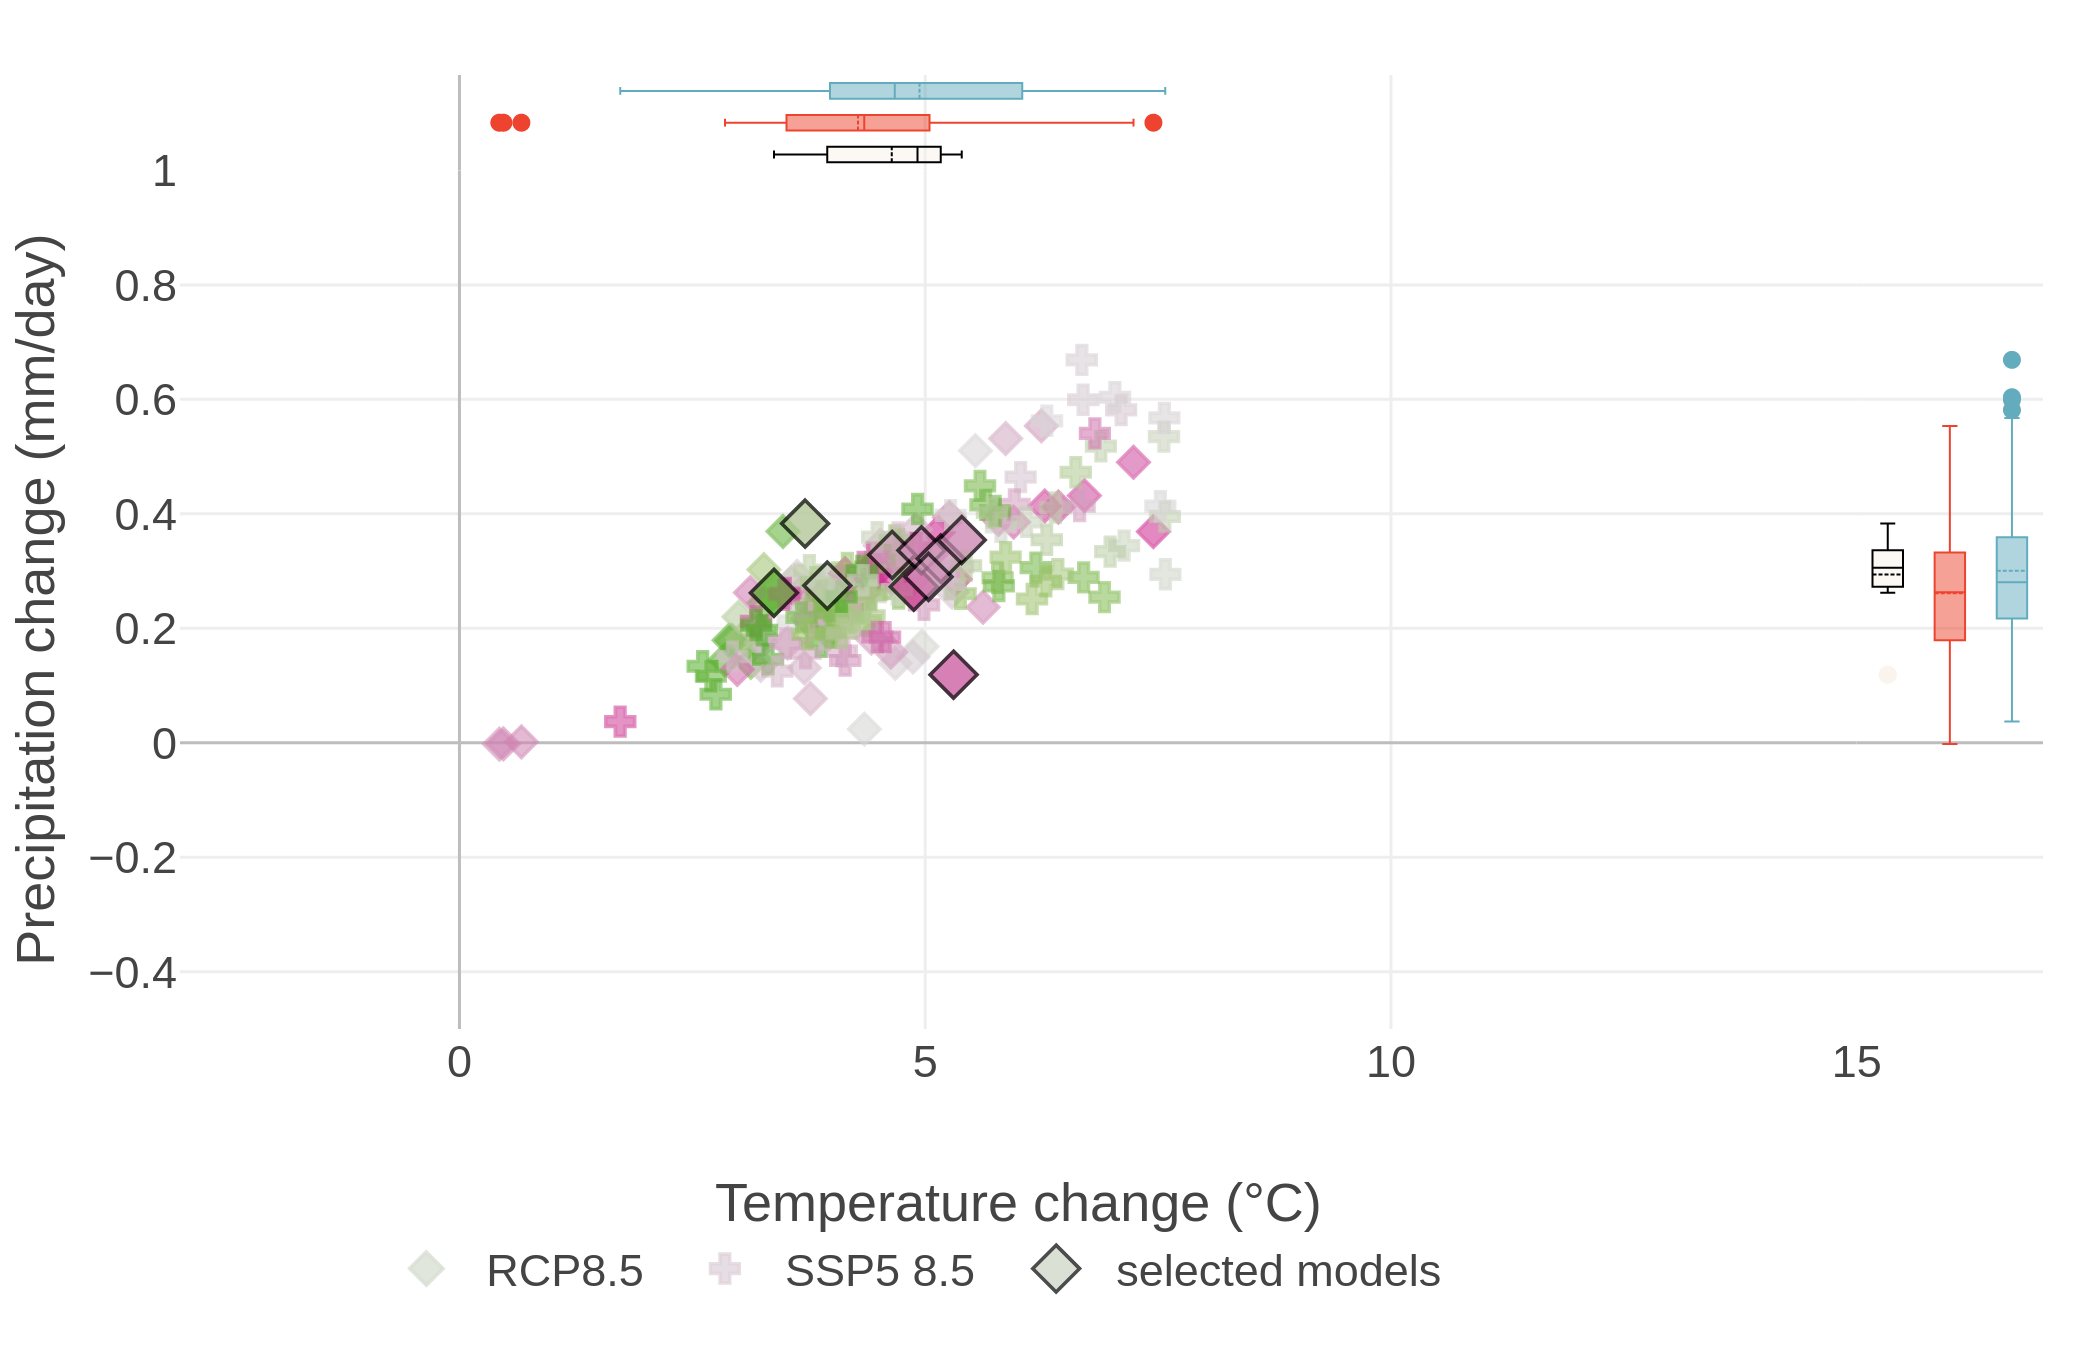
\includegraphics{fig/GCMevalNorthEuropeBestModels.png}

The global climate models indicate quite a range of future outcomes in terms of
precipitation and temperature.
To account for that, regional scenarios need to use fairly large multi-model ensembles.

\href{https://gcmeval.met.no/}{GCM-eval}

\hypertarget{measuering-forcings}{%
\subsection{Measuering Forcings}\label{measuering-forcings}}

Earth is on a budget -- an energy budget. Our planet is constantly trying to balance the flow of energy in and out of Earth's system. But human activities are throwing that off balance, causing our planet to warm in response.

Adding more components that absorb radiation -- like greenhouse gases -- or removing those that reflect it -- like aerosols -- throws off Earth's energy balance, and causes more energy to be absorbed by Earth instead of escaping into space. This is called a radiative forcing, and it's the dominant way human activities are affecting the climate.

limate modelling predicts that human activities are causing the release of greenhouse gases and aerosols that are affecting Earth's energy budget. Now, a NASA study has confirmed these predictions with direct observations for the first time: radiative forcings are increasing due to human actions, affecting the planet's energy balance and ultimately causing climate change.
The \href{https://agupubs.onlinelibrary.wiley.com/doi/10.1029/2020GL091585}{paper} was published online March 25, 2021, in the journal Geophysical Research Letters.

NASA's Clouds and the Earth's Radiant Energy System (CERES) project studies the flow of radiation at the top of Earth's atmosphere. A series of CERES instruments have continuously flown on satellites since 1997. Each measures how much energy enters Earth's system and how much leaves, giving the overall net change in radiation. That data, in combination with other data sources such as ocean heat measurements, shows that there's an energy imbalance on our planet.
But it doesn't tell us what factors are causing changes in the energy balance.

This study used a new technique to parse out how much of the total energy change is caused by humans. The researchers calculated how much of the imbalance was caused by fluctuations in factors that are often naturally occurring, such as water vapor, clouds, temperature and surface albedo (essentially the brightness or reflectivity of Earth's surface).
The researchers calculated the energy change caused by each of these natural factors, then subtracted the values from the total. The portion leftover is the radiative forcing.

The team found that human activities have caused the radiative forcing on Earth to increase by about 0.5 Watts per square meter from 2003 to 2018. The increase is mostly from greenhouse gases emissions from things like power generation, transport and industrial manufacturing. Reduced reflective aerosols are also contributing to the imbalance.

\href{https://www.nasa.gov/feature/goddard/2021/direct-observations-confirm-that-humans-are-throwing-earth-s-energy-budget-off-balance}{NASA Goddard Direct Observations of Forcings}

\hypertarget{part-measurements}{%
\part{Measurements}\label{part-measurements}}

\hypertarget{attribution}{%
\chapter{Attribution}\label{attribution}}

For too long, weather's randomness has kept events such as these from being blamed squarely on climate change. Reporters in the late 1990s and early 2000s would ask climate scientists about climate change's role in a weather-related disaster. All we could say was that we'd expect to see more of these events. Now, we can specify increased chances for specific events. This extends to forecasts: we can identify the places that are more likely to see wildfires, mudslides and fish die-offs. Such calculations dent both climate denial and a false sense of security. They take away the argument that `extreme weather happens anyway, so we don't need to worry about it'. Extreme weather happens --- and these metrics pinpoint what is becoming more likely, by how much and why.

\href{https://www.nature.com/articles/d41586-021-00185-x}{Betts (2021) Nature}

\href{https://www.ametsoc.org/ams/index.cfm/publications/bulletin-of-the-american-meteorological-society-bams/explaining-extreme-events-from-a-climate-perspective/}{Ametsoc (2021) Explaining Extreme Weather}
\href{pdf/Ametsoc_2021_Explaining_Extreme_2019.pdf}{(pdf)}

\hypertarget{map-of-attribution-studies}{%
\section{Map of Attribution Studies}\label{map-of-attribution-studies}}

Known as ``extreme event attribution'', the field has gained momentum, not only in the science world, but also in the media and public imagination. These studies have the power to link the seemingly abstract concept of climate change with personal and tangible experiences of the weather.

Scientists have published more than 300 peer-reviewed studies looking at weather extremes around the world, from wildfires in Alaska (pdf) and hurricanes in the Caribbean to flooding in France and heatwaves in China. The result is mounting evidence that human activity is raising the risk of some types of extreme weather, especially those linked to heat.

To track how the evidence on this fast-moving topic is stacking up, Carbon Brief has mapped -- to the best of our knowledge -- every extreme-weather attribution study published to date.

The map above shows 355 extreme weather events and trends across the globe for which scientists have carried out attribution studies.

\href{https://www.carbonbrief.org/mapped-how-climate-change-affects-extreme-weather-around-the-world}{Carbon BriefMap}

\hypertarget{bottom-trawling-co2-release}{%
\section{Bottom Trawling CO2 release}\label{bottom-trawling-co2-release}}

\emph{Time Magzine: How Industrial Fishing Creates More CO2 Emissions Than Air Travel}

Bottom trawling is responsible for one gigaton of carbon emissions a year---a higher annual total than (pre-pandemic) aviation emissions. Not only does the practice contribute to climate change, it is extremely damaging to ocean biodiversity---the ``equivalent of ploughing an old-growth forest into the ground, over and over and over again until there is nothing left''

Bottom trawling is also one of the least cost effective methods of fishing. Most locations have been trawled so many times, there is little left worth catching.
Without government subsidies, no one would be making a penny.

Refuting a long-held view that ocean protection harms fisheries, the study found that well placed marine protected areas (MPAs) that ban fishing would actually boost the production of marine life by functioning as fish nurseries and biodiversity generators capable of seeding stocks elsewhere.

\emph{Sala}

Marine sediments are the largest pool of organic carbon on the planet and a crucial reservoir for long-term storage29. If left undisturbed, organic carbon stored in marine sediments can remain there for millen-nia30. However, disturbance of these carbon stores can re-mineralize sed-imentary carbon to CO2, which is likely to increase ocean acidification, reduce the buffering capacityof the ocean and potentially add to the build-up of atmospheric CO2

Using satellite-inferred information on fishing activity by industrial trawlers and dredgers between 2016 and 2019, aggregated at a reso-lution of 1km2, we estimate that 4.9million km2 or 1.3\% of the global ocean is trawled each year. This disturbance to the seafloor results in an estimated 1.47Pg of aqueous CO2 emissions, owing to increased carbon metabolism in the sediment in the first year after trawling. If trawling continues in subsequent years, emissions decline as sediment
carbon stocks become exhausted. However, after 9 years of continuous trawling, emissions stabilize at around 40\% of the first year's emissions, or around 0.58Pg CO2 (Supplementary Fig.35). If the intensity and footprint of trawling remains constant, we estimate that sediment carbon emissions will continue at approximately 0.58Pg CO2 for up to around 400 years of trawling, after which all of the sediments in the top metre are depleted. Although 1.47Pg CO2 represents only 0.02\% of total marine sedimentary carbon, it is equivalent to 15--20\% of the atmospheric CO2 absorbed by the ocean each year32,33, and is compara-ble to estimates of carbon loss in terrestrial soils caused by farming34. Although an unknown fraction of the aqueous CO2 is emitted to the atmosphere, the increase in CO2 in the water column and sediment pore waters can have far-reaching and complex effects on marine carbon cycling, primary productivity and biodiversity.

\href{https://time.com/5947430/bottom-trawling-carbon-emissions-study/}{Time Magzine}
\href{https://www.bbc.com/news/science-environment-56430542}{BBC}
\href{https://www.nature.com/articles/s41586-021-03371-z.epdf?sharing_token=6Sow3BIdqBYvlWAiGEDpk9RgN0jAjWel9jnR3ZoTv0MwjSp_dqdYRo11ccDn9dqPW5D1xJuK8fpT__q4KFNUwr3chDwJyG9IO5W1aWFy5onfZKtxUPkvQTnzNtoVopyg-N66E6j3SdEzqNh2UnnVHpANtYD9CYy7I3QNIz6iI184RD1jaDt2fU8Yl8bdsQppKG7J6tfBiSTN74eTrygUTMPeqTv4M1289Ys38rtf2Cu5Gfo8iuQxzcCwuSri_N3NIdmY-iR2Af8IOP_F9-p_RA\%3D\%3D\&tracking_referrer=time.com}{Sala (2021) Protecting the global ocean for biodiversity, food and climate - Nature Share}

\hypertarget{company-attribution}{%
\section{Company Attribution}\label{company-attribution}}

A 2017 report by the Carbon Disclosure Project showed that 100 companies have been responsible for 71 per cent of global emissions since 1988. In 2019, a similar study from the Climate Accountability Institute found that just 20 companies were responsible for 35 per cent of all energy-related carbon dioxide and methane worldwide since 1965.

\href{https://tribunemag.co.uk/2021/03/paper-straws-are-not-enough}{Sultana}

\hypertarget{carbon-budget}{%
\chapter{Carbon Budget}\label{carbon-budget}}

\begin{quote}
The temperature response for a 1.5°C scenario has a huge uncertainty \& this propagates to the uncertainty in the carbon budget.
To say ``the remaining carbon budget for 1.5°C is 440 GtCO₂'' {[}add favorite number{]} is highly misleading
Taking a narrow 67--33\% range, the value is 230--670 GtCO₂, but full range (left) could be −1000 - 2000 GtCO₂\ldots{} (yes, could be negative or huge)
(Glen Peters)
\end{quote}

\emph{Memo Matthews:}

The remaining carbon budget quantifies the future CO 2 emissions to limit global warming
below a desired level. Carbon budgets are subject to uncertainty in the Transient Climate
Response to Cumulative CO 2 Emissions (TCRE), as well as to non-CO 2 climate influences.
We estimate a median TCRE of 0.44 °C and 5--95\% range of 0.32--0.62 °C per 1000 GtCO 2
emitted. Considering only geophysical uncertainties, our median estimate of the 1.5 °C
remaining carbon budget is 440 GtCO 2 from 2020 onwards, with a range of 230--670
GtCO 2 , (for a 67--33\% chance of not exceeding the target). Additional socioeconomic
uncertainty related to human decisions regarding future non-CO 2 emissions scenarios can
further shift the median 1.5 °C remaining carbon budget by ±170 GtCO 2 .

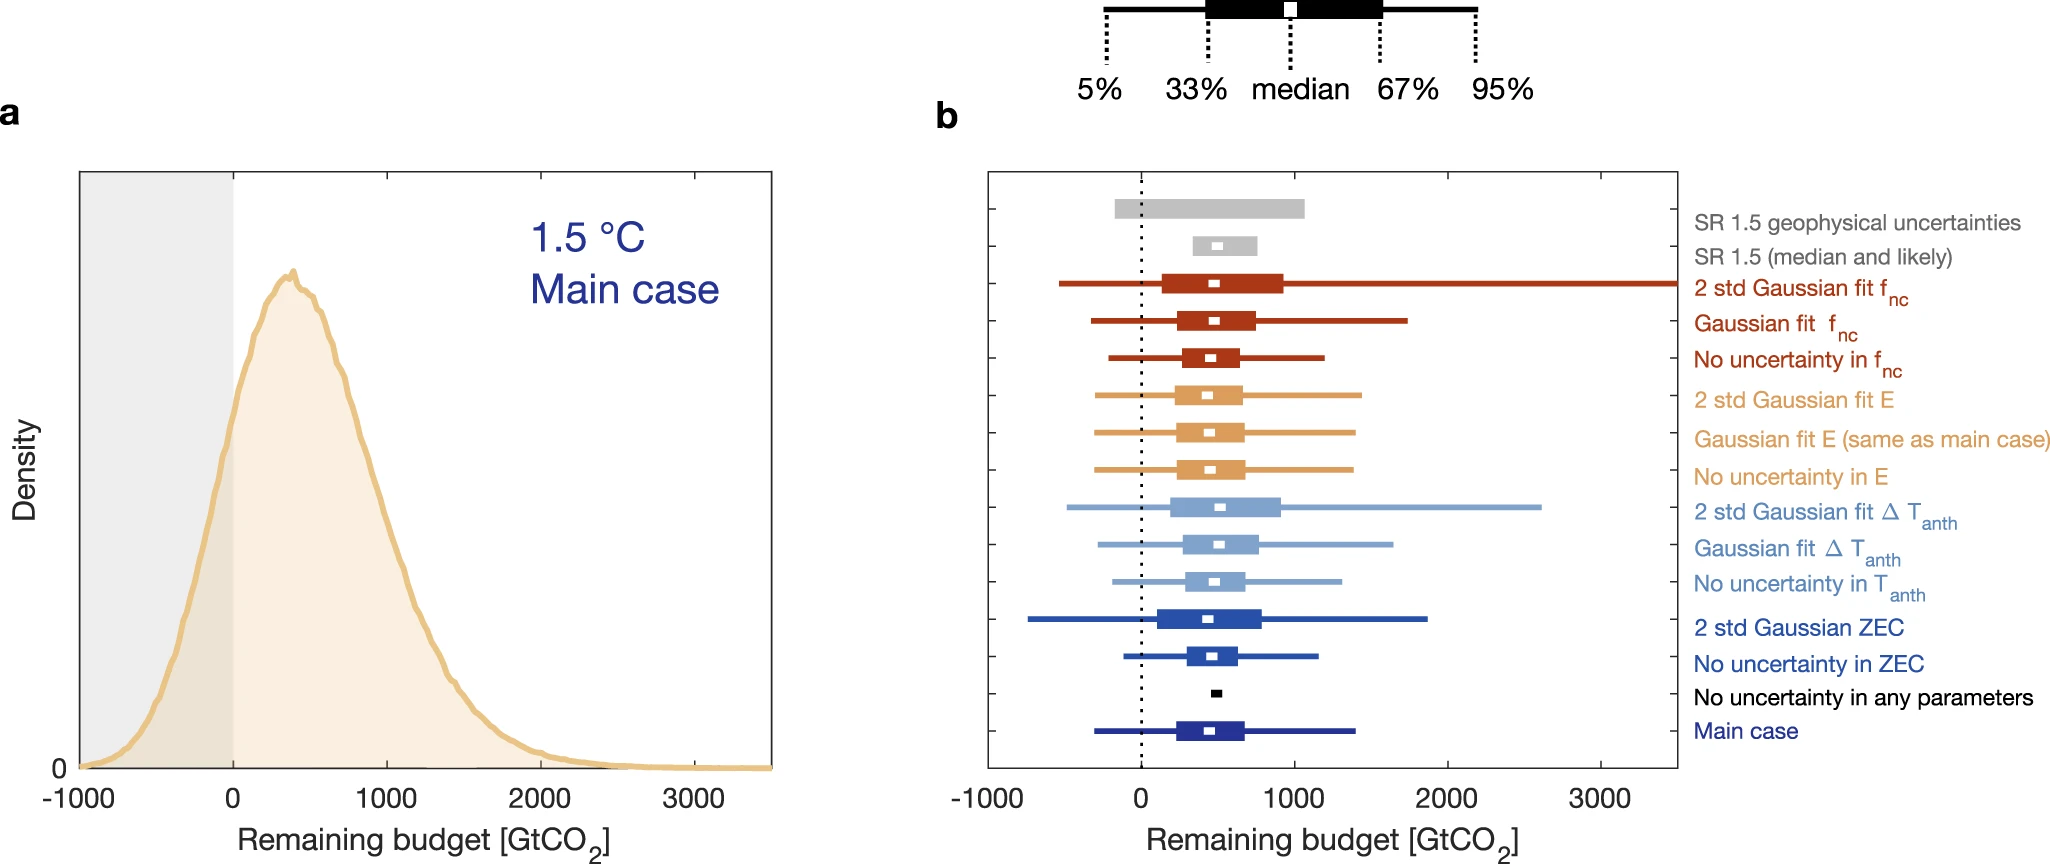
\includegraphics{fig/carbon_budget.png}

Remaining carbon budgets (RCBs) represent the future
cumulative CO 2 emissions that would be consistent with
keeping global warming to a specified level.
Despite being conceptually simple, RCBs have been
defined and estimated in various ways and with many different
underlying assumptions, resulting in a wide range of
``best estimates'' across different studies 2 . Moreover, most of these
estimates of remaining budgets account for only a subset of the
relevant uncertain processes and often omit the contribution of
key uncertain processes (such as permafrost thaw or future
scenario uncertainty, among others)

Median TCRE estimate is 0.44 °C per 1000 GtCO2 , with a 5--95\%
range of 0.32--0.62 °C per 1000 GtCO2

A stronger constraint on the left-hand side of the distribution (low
TCRE values, with sharply increasing probability above 0.25 °C/
1000 GtCO 2 ), while the right-hand side of this distribution has a
wider tail. This right-skewed distribution shape of our
observationally-constrained TCRE estimate is physically related
to the possibility of a large negative aerosol forcing

Median RCB for 1.5 °C is 440 GtCO2 from 2020
onwards, representing a 50\% chance of stabilising warming at or
below 1.5 °C.
The corresponding budget for a 67\% chance of remaining below the target is
230 GtCO2 from the year 2020 onwards.

\href{https://www.nature.com/articles/s43247-020-00064-9}{Matthews(2021) Carbon Budget Uncertainties}
\href{pdf/Matthews_2021_Carbon_Budget_Uncertainties.pdf}{(pdf)}

\hypertarget{net-zero}{%
\section{Net-zero}\label{net-zero}}

\emph{Disaster looms if big finance is allowed to game the carbon offsetting markets to achieve `net zero' emissions.}

\emph{Net zero increasingly involves highly questionable carbon accounting. As a result, the new politics swirling around net zero targets is rapidly becoming a confusing and dangerous mix of pragmatism, self-delusion and weapons-grade greenwash.}

The science of net zero is simple: every sector of every country in the world needs to be, on average, zero emissions. We know how to do this for electricity, cars, buildings and even a lot of heavy industry. But in certain areas, including air travel and some agricultural emissions, there is no prospect of getting to zero emissions in the near future. For these residual emissions, greenhouse gasses will need to be sucked out of the atmosphere at the same rate as they are added, so that, on average, there are net zero emissions.

The science of net zero is simple: every sector of every country in the world needs to be, on average, zero emissions. We know how to do this for electricity, cars, buildings and even a lot of heavy industry. But in certain areas, including air travel and some agricultural emissions, there is no prospect of getting to zero emissions in the near future. For these residual emissions, greenhouse gasses will need to be sucked out of the atmosphere at the same rate as they are added, so that, on average, there are net zero emissions.

Making this work requires carbon removal, also known as ``negative emissions''. This can be low-tech, like restoring forests, as this takes carbon out of the atmosphere and stores it in trees. Or it can be hi-tech, like using chemicals to strip carbon dioxide from the atmosphere and then pumping it deep underground into safe geological storage. In theory this is all fine, as pragmatically some carbon removal is needed to balance hard-to-reduce emissions: but negative emissions and offsetting alone are not a route to net zero.

In practice, by believing in the promise of these methods, we are too often deceiving ourselves, in three major ways. The first is an unrealistic overreliance on carbon removal to preserve the status quo.
Critically, there is far too little land to plant enough trees to counter today's emissions, and large-scale hi-tech methods do not yet exist.
The second deception is in offsetting against notional emissions trajectories instead of removing carbon from the atmosphere.Offsetting needs to be used to remove carbon dioxide from the atmosphere to counter difficult-to-remove emissions, and not just be an enabler of business-as-nearly-usual.
The third deception comes from not getting what you think you're paying for in the self-regulated global carbon market. The commercial carbon offset concept relies on ``additionality'' -- that money paid then reduces emissions or captures carbon that would not otherwise have happened.
The offsets market is awash with old legacy carbon credits where that assumption is violated.

If such deceptions remain, disaster looms. Big finance, led by Carney, is planning to massively expand carbon markets. Conceivably, new carbon-based financial products could boom, with little impact on emissions. Just like the sub-prime crisis, few will understand what they bought, and another globe-spanning crash could sweep the world, compounding economic and climate crises causing mass suffering, as we realise again that the Earth owes us nothing. Nature doesn't do bailouts.

\href{https://www.theguardian.com/commentisfree/2021/mar/03/climate-crisis-carbon-accounting-tricks-big-finance}{Lewis (Guardian)}

\hypertarget{climate-sensitivity}{%
\chapter{Climate Sensitivity}\label{climate-sensitivity}}

\hypertarget{climate-feedbacks}{%
\section{Climate Feedbacks}\label{climate-feedbacks}}

\emph{Abstract Heinze}
Earth system models (ESMs) are key tools for providing climate projections under different sce-
narios of human-induced forcing. ESMs include a large number of additional processes and feedbacks such as
biogeochemical cycles that traditional physical climate models do not consider. Yet, some processes such as
cloud dynamics and ecosystem functional response still have fairly high uncertainties. In this article, we present
an overview of climate feedbacks for Earth system components currently included in state-of-the-art ESMs and
discuss the challenges to evaluate and quantify them. Uncertainties in feedback quantification arise from the in-
terdependencies of biogeochemical matter fluxes and physical properties, the spatial and temporal heterogeneity
of processes, and the lack of long-term continuous observational data to constrain them. We present an outlook
for promising approaches that can help to quantify and to constrain the large number of feedbacks in ESMs in
the future. The target group for this article includes generalists with a background in natural sciences and an
interest in climate change as well as experts working in interdisciplinary climate research (researchers, lecturers,
and students). This study updates and significantly expands upon the last comprehensive overview of climate
feedbacks in ESMs, which was produced 15 years ago (NRC, 2003).

\href{https://www.researchgate.net/publication/334387499_ESD_Reviews_Climate_feedbacks_in_the_Earth_system_and_prospects_for_their_evaluation}{Heinze (2019) Climate Feedbacks}
\href{pdf/Heinze_2019_Climate_Feedbacks.pdf}{(pdf)}

\hypertarget{ecs---equilibrium-climate-sensitivity}{%
\section{ECS - Equilibrium Climate Sensitivity}\label{ecs---equilibrium-climate-sensitivity}}

\emph{ECS}

Climate sensitivity is defined as the equilibrium change in global and annual mean
surface air temperature, \(\Delta T\), due to an increment in
downward radiative flux, \(\Delta R_{f}\) ,
that would result from sustained doubling of atmospheric \(CO_2\) over its
preindustrial value (2 x \(CO_2\) ).

Studies based, on observations, energy balance models, temperature reconstructions,
and global climate models (GCMs) have found that the probability
density distribution of \(\Delta T\) is peaked in the range
2.0°C ≤ \(\Delta T\) ≤ 4.5°C, with a long tail of small but
finite probabilities of very large temperature increases.

An important parameter in climate science is
the equilibrium or long-run response in the global mean surface temperature
to a doubling of atmospheric carbon dioxide.

In the climate science community, this is called
the equilibrium climate sensitivity ECS.
With reference to climate models, this is calculated as
the increase in average surface temperature with a doubled CO2 concentration
relative to a path with the pre-industrial CO2 concentration.
This parameter also plays a key role in the geophysical components
in the IAMs.

Given the importance of the ECS in climate science,
there is an extensive literature estimating probability density functions.
These pdfs are generally based on climate models, the instrumental
records over the last century or so, paleoclimatic data such
as estimated temperature and radiative forcings over ice-age intervals,
and the results of volcanic eruptions.
Much of the literature estimates a probability density function
using a single line of evidence,
but a few papers synthesize different studies or different kinds of evidence.

The IPCC Fifth Assessment report (AR5) reviewed the literature
quantifying uncertainty in the ECS and highlighted
five recent papers using multiple lines of evidence (IPCC, 2014).
Each paper used a Bayesian approach to update a prior distribution
based on previous evidence
(the prior evidence usually drawn from instrumental records or a climate model)
to calculate the posterior probability density function.

\href{https://globalchange.mit.edu/publication/16235}{Gilligham (2015) Modelling Uncertainty}
\href{pdf/Gillingham_2015_Modelling_Uncertainty.pdf}{(pdf)}

\hypertarget{roe-and-baker-distribution}{%
\subsection{Roe and Baker Distribution}\label{roe-and-baker-distribution}}

\emph{Abstract}

Uncertainties in projections of future climate change have not lessened substantially in past
decades. Both models and observations yield broad probability distributions for long-term
increases in global mean temperature expected from the doubling of atmospheric carbon dioxide,
with small but finite probabilities of very large increases. We show that the shape of these
probability distributions is an inevitable and general consequence of the nature of the climate
system, and we derive a simple analytic form for the shape that fits recent published distributions
very well. We show that the breadth of the distribution and, in particular, the probability of
large temperature increases are relatively insensitive to decreases in uncertainties associated with
the underlying climate processes.

\emph{Memo Roe and Baker}

What determines the distribution shape of ECS and in particular, the high \(\Delta T\) tail?
To what extent we can decrease the distribution width?

Climate consists of a set of highly coupled, tightly interacting physical processes.
Understanding these physical processes is a massive
task that will always be subject to uncertainty.
How do the uncertainties in the physical processes translate into an uncertainty in climate
sensitivity?

Explanations for the range of
predictions of DT, summarized in (14), have
focused on
(i) uncertainties in our understanding of the individual physical processes
(in particular, those associated with clouds),
(ii) complex interactions among the individual processes, and
(iii) the chaotic, turbulent nature of the climate system, which may give rise to
thresholds, bifurcations, and other discontinuities, and which
remains poorly understood on a theoretical level.
We show here that the explanation is far more fundamental than any of these.

We use the framework of feedback analysis to examine the relationship between the
uncertainties in the individual physical processes and the ensuing shape of
the probability distribution of \(\Delta T\).
Because we are considering an equilibrium temperature rise, we consider only
time-independent processes.

\href{https://www.semanticscholar.org/paper/Why-Is-Climate-Sensitivity-So-Unpredictable-Roe-Baker/9a0c81f6887db897000dbce576b139a486f62c77}{Roe and Baker (2007) Climate Sensitivity}
\href{pdf/Roe_Baker_2007_Climate_Sensitivity.pdf}{(pdf)}

\emph{Memo Hannart}

RB addressed these questions using rather simple
theoretical considerations and reached the conclusion that
reducing uncertainties on climate feedbacks and underlying
climate processes will not yield a large reduction in the
envelope of climate sensitivity. In this letter, we revisit the
premises of this conclusion. We show that it results from a
mathematical artifact caused by a peculiar definition of
uncertainty used by these authors.

Reducing inter-model spread on
feedbacks does in fact induce a reduction of uncertainty on
climate sensitivity, almost proportionally.
Therefore, following Roe and Baker assumptions, climate sensitivity is actually
not so unpredictable.

The main originality of RB07 approach consists in analyzing
explicitly the way uncertainties on \(f\), due to a limited
understanding of their underlying physical processes, prop-
agates into uncertainties on \(\Delta T\): assuming \(f\) is a random
variable with mean \(f\) and standard deviation \(\sigma_f\) , RB07 uses
this simple probabilistic model to highlight several fundamental
properties of uncertainty propagation from feedbacks
to climate sensitivity. The most prominent conclusion of this
analysis is that reducing uncertainties on \(f\) does not yield a
large reduction in the uncertainty of \(\Delta T\), and thus that
improvements in the understanding of physical processes
will not yield large reductions in the envelope of future
climate projections.
We show that this conclusion is a mathematical artifact
with no connection whatsoever to climate.

RB07 uses the feedback analysis framework.
Denoting \(\Delta T_0\) the Planck temperature response to the radiative
perturbation and \(f\) the feedback gain (RB07 refers to it as
feedback factor), they obtain:

\[\Delta T = \frac{\Delta T_0}{1 - f}\]

RB07 then assumes uncertainty on Planck response to be
negligible so that the entire spread on \(\Delta T\) results from the
uncertainty on the global feedback gain \(f\). To model this
uncertainty, RB07 assumes that \(f\) follows a Gaussian
distribution with mean \(\overline{f}\) , standard deviation \(\sigma_f\) and implicit
truncation for \(f\) \textgreater{} 1.
Then, they derive an exact expression of the distribution of \(\Delta T\).
This simple probabilistic climatic model is used by RB07 to analyze the
way uncertainties on \(f\), due to a limited understanding of
underlying physical processes, propagates into uncertainties
on \(\Delta T\). Their analysis highlights two fundamental properties:

\begin{enumerate}
\def\labelenumi{\arabic{enumi}.}
\item
  \emph{Amplification}: The term in \(\frac{1}{1-f}\)
  amplifies uncertainty on feedbacks, all the more intensely as
  \(f\) is close to (though lower than) one. Small uncertainties on
  feedbacks are thus converted in large uncertainties on the
  rise of temperature.
\item
  \emph{Insensitivity}: reducing uncertainty on \(f\) has
  little effect in reducing uncertainty on \(\Delta T\),
  also stated as the breadth of the distribution of \(\Delta T\)
  is relatively insensitive to decreases in \(\sigma_f\).
\end{enumerate}

We are puzzled by the second property, that is,
the claimed insensitivity of uncertainty on \(\Delta T\) to uncertainty on feedbacks.
The reason why one may find this second assertion puzzling,
is that it intuitively seems to contradict the first.

While the probability \(P(\Delta T \in [4.5°C, 8°C])\) may be of interest practically,
this metric is irrelevant to describe \emph{the breadth of the
distribution of climate sensitivity} which was RB07 explicit intent.
To address this question, any measure of distribution
spread chosen amongst those classically used in Descriptive
Statistics is more appropriate.

(Hugo Mathjax don't render correctly here:?? OK in rpad !! OK in mathjaxtest!!)
With such measures when the spread of feedback parameter \(S_f\) decreases,
the resulting spread of climate sensitivity \(S_{\Delta T}\) values also decreases.
Further the decrease is approximately linear for
\(S_f\) small and tends to be steeper for larger values of \(S_{f}\) .

\href{https://agupubs.onlinelibrary.wiley.com/doi/full/10.1029/2009GL039640}{Hannart on RB}
\href{pdf/Hannart_2009_ECS_not_so_Unpredictable.pdf}{(pdf)}

\href{https://github.com/rtol/roebaker}{Tol: RB-fitting Github}

\emph{Memo Jules and James}
Roe and Baker have attempted to justify the pdfs that have been generated
as not only reasonable, but inevitable on theoretical grounds

RB's basic point is that if ``feedback'' \(f\) is considered to be Gaussian, then
sensitivity = \(\lambda_0/(1-f)\) is going to be skewed, which seems fair enough.

Where I part company with them is when they claim that this gives rise to some
fundamental and substantial difficulty in generating more precise estimates
of climate sensitivity, and also that it explains
the apparent lack of progress in improving on the long-standing
1979 Charney report estimate of 1.5-4.5C at only the ``likely'' level.

Stoat's complaints also seem pertinent:
\(f\) cannot really be a true Gaussian,
unless one is willing to seriously consider large negative sensitivity,
and even though a Gaussian is a widespread and often reasonable distribution,
it is hard to find any theoretical or practical basis for
a Gaussian abruptly truncated at 1.

I can think of several alternative theories as to
why the uncertainty in the IPCC estimate has not reduced.
The probabilistic methods generally used to generate these long-tailed pdfs
are essentially pathological in their use of a uniform prior
(under the erroneous belief that this represents ``ignorance''),
together with only looking at one small subset of the pertinent data at a time,
and therefore do not give results that can credibly represent
the opinions of informed scientists.

There may also be the sociological effect of this range as some sort of anchoring device, which people are reluctant to change despite its rather shaky origins. Ramping up uncertainty (at least at the high end) is a handy lever for those who argue for strong mitigation, and it would also be naive to ignore the fact that scientists working in this area benefit from its prominence.

\href{http://julesandjames.blogspot.com/2007/10/roe-and-baker.html}{Jules and James: Comment on RB}

\emph{Memo Gillingham}

Note that the US government used a version of the Roe and Baker distribution
calibrated to three constraints from the IPCC
for its uncertainty estimates (IAWG, 2010).
Specifically, the IAWG Report modified the original Roe and Baker distribution
to assume that the median value is 3.0°C,
the probability of being between 2 and 4.5°C is two-thirds,
and there is no mass below zero or above 10°C.
The modified Roe and Baker distribution has a higher mean ECS than
any of the models (3.5°C) and
a much higher dispersion (1.6°C as compared to 0.84°C from Olsen et al.~2012).

\href{https://globalchange.mit.edu/publication/16235}{Gilligham (2015) Modelling Uncertainty}
\href{pdf/Gillingham_2015_Modelling_Uncertainty.pdf}{(pdf)}

\hypertarget{gcm-based-approach}{%
\subsection{GCM based Approach}\label{gcm-based-approach}}

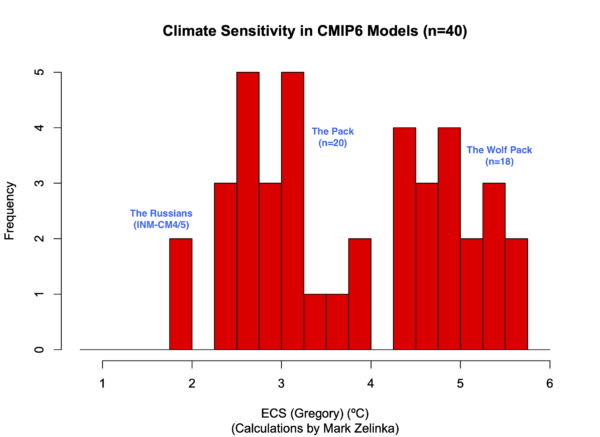
\includegraphics{fig/Gavin_2020_cmip6_ecs.png}

\href{http://www.realclimate.org/index.php/archives/2019/11/sensitive-but-unclassified/}{Gavin (2019) RealClimate (Part 1)}

\href{http://www.realclimate.org/index.php/archives/2020/06/sensitive-but-unclassified-part-ii/}{Gavin (2020) RealClimate (Part 2)}

\hypertarget{gcm-free-approach}{%
\subsection{GCM free Approach}\label{gcm-free-approach}}

\emph{Memo}

\begin{itemize}
\tightlist
\item
  GCM free approach
\end{itemize}

The atmosphere is a complex system involving turbulent
processes operating over a wide range of scales starting
from millimeters at the Kolmogorov dissipation scale up
to the size of the Earth, spanning over 10 orders of magni-
tudes in space.

The dynamics are sensitive to initial conditions and there are
deterministic predictability limits that
are roughly equal to the eddy turn-over time (lifetime) of
structures.

For planetary scale structures in the atmosphere,
the overall deterministic prediction limit of about 10 days
corresponds to the scaling transition timescale τ w from the
weather regime to the macroweather regime.

The atmospheric components of GCMs exhibit the same
weather-macroweather scaling transition as the atmosphere
and similar predictability limits. Beyond this horizon, the
internal variability has to be interpreted stochastically so
that a single GCM run is only one realization of the random
process; at these timescales, weather models effectively
become stochastic macroweather generators. For projec-
tions over multi-decadal timescales and beyond, multi-model
ensembles (MME) that include several models are used. The
mean of the MME is taken to obtain the deterministic forced
component of temperature variability and average out the
internal variability (Collins et al.~2013).

Emergent properties of the Earth's climate, i.e.~proper-
ties which are not specified a priori, are then inferred from
GCM simulations.

The equilibrium climate sensitivity (ECS)
is such a property; it refers to the expected temperature
change after an infinitely long time following a doubling in
carbon dioxide ( CO 2 ) atmospheric concentration.

Another is the transient climate response (TCR), which is defined
as the change in temperature after a gradual doubling of
CO 2 atmospheric concentration over 70 years at a rate of
1\% per year.

However, it is not clear whether such emer-
gent properties from computational models can be taken as
genuine features of the natural world.

The difficulty is that
each GCM has its own climate (``structural uncertainty'')
and this leads to very large discrepancies in ECS and TCR
between GCMs; this underscores the need for qualitatively
different approaches which can narrow down the properties
of the real climate directly from observations.

The ecological consequences of global warming could be dire;
therefore, better constraining climate sensitivity is of
utmost importance in order to meet the urgency of adjusting
economical and environmental policies.

Multidecadal climate projections rely almost exclusively
on deterministic global climate models (GCMs) in spite of
the fact that there are still very large structural uncertainties
between Coupled Model Intercomparison Project phase 5
(CMIP5) GCMs, i.e.~each has its own climate, rather than
the real world climate.

Climate skeptics have argued that
IPCC projections are untrustworthy precisely because they
are entirely GCM based.
While this conclusion is unwarranted, it underscores the need for
independent and qualitatively different approaches.
It is therefore significant that
the alternative GCM-free approach we present here yields
comparable results albeit with smaller uncertainty.

According to our projections made to 2100, to avert a 1.5
K warming, future emissions will be required to undergo
drastic cuts similar to RCP 2.6, for which we found a 46\%
probability to remain under the said limit; it is virtually cer-
tain that RCP 4.5 and RCP 8.5-like futures would overshoot.

Even a 2.0 K warming limit would surely be surpassed by
2100 under RCP 8.5 and probably also under RCP 4.5, with
only a 6\% chance of remaining under the limit. The safest
option remains RCP 2.6 which we project to remain under
2.0 K with very high confidence. The question remains
whether it is at all realistic given that it relies strongly on
the massive deployment of speculative negative emission
technologies.

On the other hand, our model has obvious limitations
since it assumes a linear stationary relationship between
forcing and temperature, neglecting nonlinear interac-
tions which could arise as the system evolves, as it cur-
rently warms.

In particular, so-called tipping points could
be reached in the coming century which would lead to a
breakdown of the linear model proposed. Such potential
behaviours are of critical value for improving future projections,
but they have not yet been observed with high confidence even in GCMs.

This underlines the need to exploit
paleoclimate archives to achieve a better understanding of
low-frequency natural variability, namely the transition scale
from the macroweather regime to the climate regime.

In this study, we have assumed the increased variability in the climate regime
to be strictly a result of forcing,
but internal modes of variability could also have a significant contribution
for longer timescales.

\href{https://climatenewsnetwork.net/seven-years-to-ground-zero-for-the-climate-crisis/}{Climate News Network}

\href{https://link.springer.com/article/10.1007/s00382-020-05521-x}{Climate Sensitivity article (Climate Dynamics)}
\href{pdf/Hebert_2020_Climate_Sensitivity_Estimates.pdf}{(pdf)}

\hypertarget{remote-sensing-of-tipping-points}{%
\section{Remote Sensing of Tipping Points}\label{remote-sensing-of-tipping-points}}

Many aspects of the climate are sensitive to small disrupting changes that could trigger an abrupt change in the system into a new stable state. Even at relatively low levels of global warming, systems that exhibit these instabilities could accelerate global warming through climate feedbacks or cause other cascading impacts. These `tipping elements', or `large-scale discontinuities in the climate system', as UNFCCC IPCC reports refer to them, have been assigned successively greater risk with each IPCC report since 2001.

Proximity to a tipping point may be indicated in remote sensing data by characteristic statistical changes.
Early warning indicators can be developed using an increasing trend in the lag-1 autocorrelation when it is correlated with an increase in variance.
Niklas Boers of the Potsdam Institute for Climate Impact Research highlighted recent work using these characteristic statistical changes to identify the reduction in a system's resilience, and has developed early warning indicators for Arctic sea-ice extent, Greenland ice sheet, Atlantic Meridional Overturning Circulation, the Amazon rainforest and the South American Monsoon system. The technique has also been applied to aquatic ecosystems and marine anoxic events.
Automatic detection of extreme events and abrupt shifts in climate datasets using edge detection algorithms.

\href{https://futureearth.org/2021/02/22/remote-sensing-of-tipping-points-in-the-climate-system/}{futureearth}

\hypertarget{decoupling}{%
\chapter{Decoupling}\label{decoupling}}

\emph{Hausfather}

\textbf{Absolute Decoupling of Economic Growth and Emissions in 32 Countries}

Between 1990 and 2019, global emissions of CO2 increased by 56\%. Historically, economic growth has been closely linked to increased energy consumption --- and increased CO2 emissions in particular --- leading some to argue that a more prosperous world is one that necessarily has more impacts on our natural environment and climate. There is a lively academic debate about our ability to ``absolutely decouple'' emissions and growth --- that is, the extent to which the adoption of clean energy technology can allow emissions to decline while economic growth continues.

Over the past 15 years, however, something has begun to change. Rather than a 21st century dominated by coal that energy modelers foresaw, global coal use peaked in 2013 and is now in structural decline.

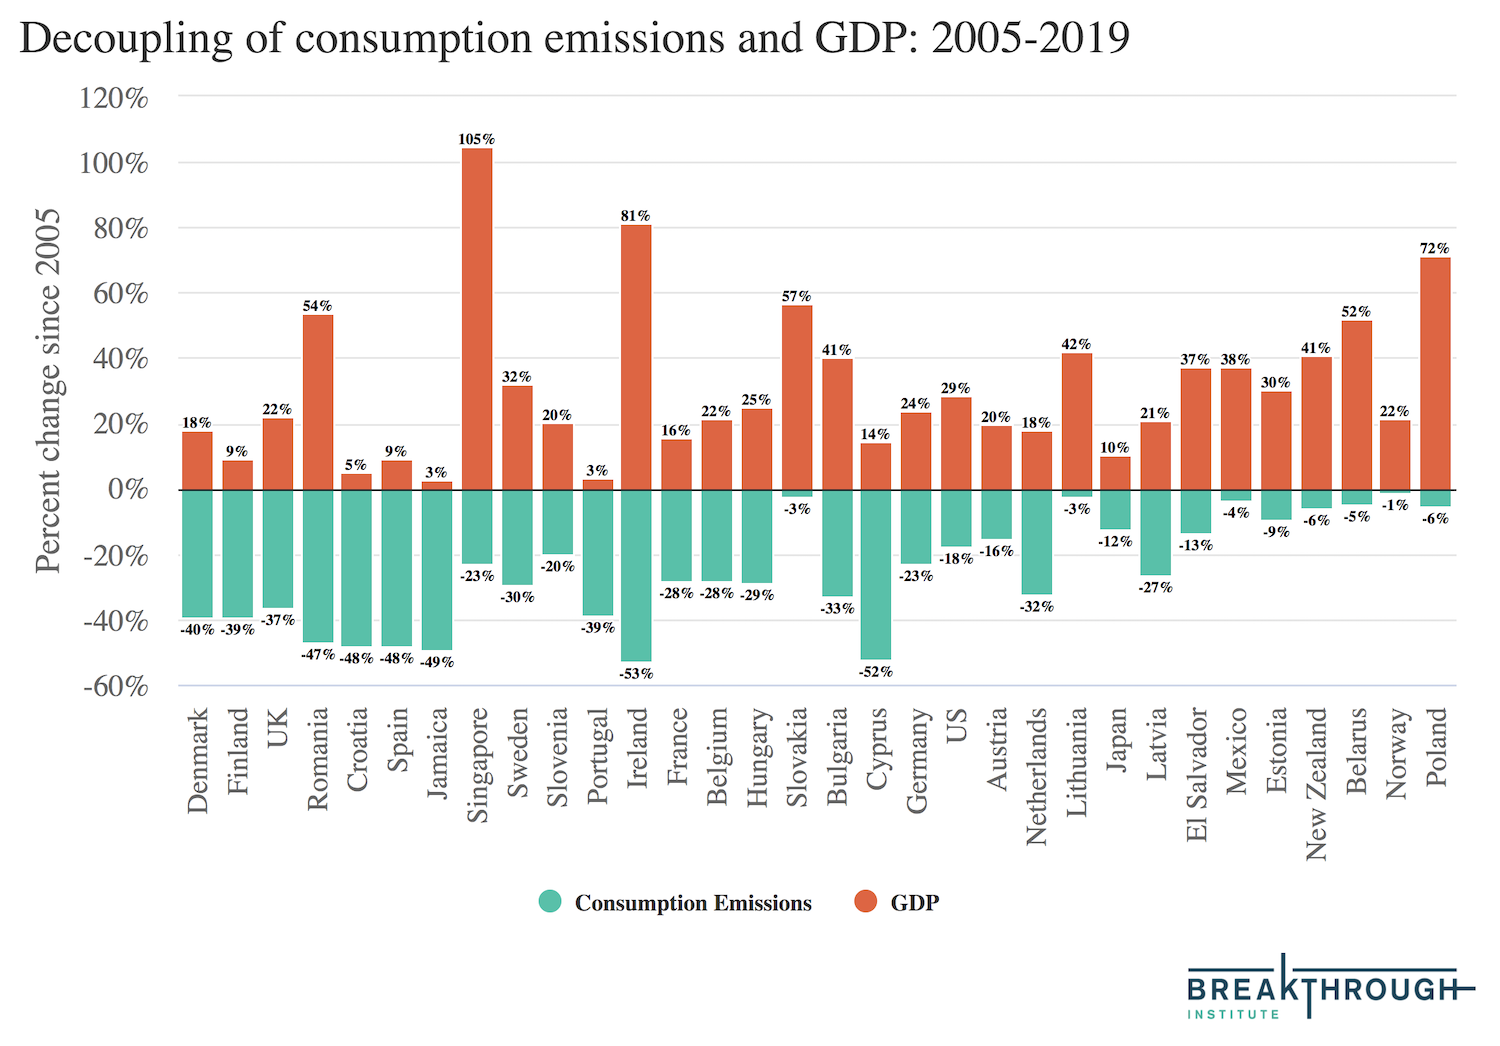
\includegraphics{fig/hausfather_decoupling.png}

These 32 countries show that it is possible to have economic growth at the same time that CO2 emissions decline, even accounting for embodied emissions in goods imported from overseas. However, these are mostly relatively wealthy countries whose economies tend to be increasingly driven by lower-energy information technology and service sectors. We have relatively few examples of low- or middle-income countries with a focus on energy-intensive manufacturing experiencing absolute decoupling to date.

Absolute decoupling is possible. There is no physical law requiring economic growth --- and broader increases in human wellbeing --- to necessarily be linked to CO2 emissions. All of the services that we rely on today that emit fossil fuels --- electricity, transportation, heating, food --- can in principle be replaced by near-zero carbon alternatives, though these are more mature in some sectors (electricity, transportation, buildings) than in others (industrial processes, agriculture).

\href{https://thebreakthrough.org/issues/energy/absolute-decoupling-of-economic-growth-and-emissions-in-32-countries}{Hausfather}

\hypertarget{paleoclimate}{%
\chapter{Paleoclimate}\label{paleoclimate}}

Earth's paleoclimate history provides guidance with a precision and reliability that climate
models cannot match. Ice cores were usually the paleoclimate data source of choice for those
scientists concerned about human-made climate change. That's understandable because ice
cores provide precise data on atmospheric composition as well as climate change.
However, ice cores cover only several hundred thousand years. That sounds like a long time, but
Earth was mostly in ice ages during that time. The ice cores encompass several interglacial
periods, but none of them were much warmer than our present global temperature.
(James Hansen: Sophies Planet Ch.40)

\hypertarget{holocen-thermal-maxima}{%
\section{Holocen Thermal Maxima}\label{holocen-thermal-maxima}}

\emph{Abstract Bova}

Proxy reconstructions from marine sediment cores indicate peak temperatures in the first half of the last and current interglacial periods (the thermal maxima of the Holocene epoch, 10,000 to 6,000 years ago, and the last interglacial period, 128,000 to 123,000 years ago) that arguably exceed modern warmth1,2,3. By contrast, climate models simulate monotonic warming throughout both periods4,5,6,7. This substantial model--data discrepancy undermines confidence in both proxy reconstructions and climate models, and inhibits a mechanistic understanding of recent climate change. Here we show that previous global reconstructions of temperature in the Holocene1,2,3 and the last interglacial period8 reflect the evolution of seasonal, rather than annual, temperatures and we develop a method of transforming them to mean annual temperatures. We further demonstrate that global mean annual sea surface temperatures have been steadily increasing since the start of the Holocene (about 12,000 years ago), first in response to retreating ice sheets (12 to 6.5 thousand years ago), and then as a result of rising greenhouse gas concentrations (0.25 ± 0.21 degrees Celsius over the past 6,500 years or so). However, mean annual temperatures during the last interglacial period were stable and warmer than estimates of temperatures during the Holocene, and we attribute this to the near-constant greenhouse gas levels and the reduced extent of ice sheets. We therefore argue that the climate of the Holocene differed from that of the last interglacial period in two ways: first, larger remnant glacial ice sheets acted to cool the early Holocene, and second, rising greenhouse gas levels in the late Holocene warmed the planet. Furthermore, our reconstructions demonstrate that the modern global temperature has exceeded annual levels over the past 12,000 years and probably approaches the warmth of the last interglacial period (128,000 to 115,000 years ago).

\href{https://www.nature.com/articles/s41586-020-03155-x}{Bova (2021) Nature (Paywall)}

\hypertarget{pattern-effect}{%
\chapter{Pattern Effect}\label{pattern-effect}}

\emph{Abtract}

Our planet's energy balance is sensitive to spatial inhomogeneities in sea surface temperature and sea ice changes, but this is typically ignored in climate projections. Here, we show the energy budget during recent decades can be closed by combining changes in effective radiative forcing, linear radiative damping and this pattern effect. The pattern effect is of comparable magnitude but opposite sign to Earth's net energy imbalance in the 2000s, indicating its importance when predicting the future climate on the basis of observations. After the pattern effect is accounted for, the best-estimate value of committed global warming at present-day forcing rises from 1.31 K (0.99--2.33 K, 5th--95th percentile) to over 2 K, and committed warming in 2100 with constant long-lived forcing increases from 1.32 K (0.94--2.03 K) to over 1.5 K, although the magnitude is sensitive to sea surface temperature dataset. Further constraints on the pattern effect are needed to reduce climate projection uncertainty.

\href{https://www.nature.com/articles/s41558-020-00955-x}{Nature article (paywall)}

\hypertarget{temperature-measurements}{%
\chapter{Temperature Measurements}\label{temperature-measurements}}

Temperatures have increased over virtually the entire planet since the mid-19th century, but the warming rate has not been the same everywhere.

When looking at the changes relative to the global average, it is clear the Arctic and land areas are warming faster than the ocean.

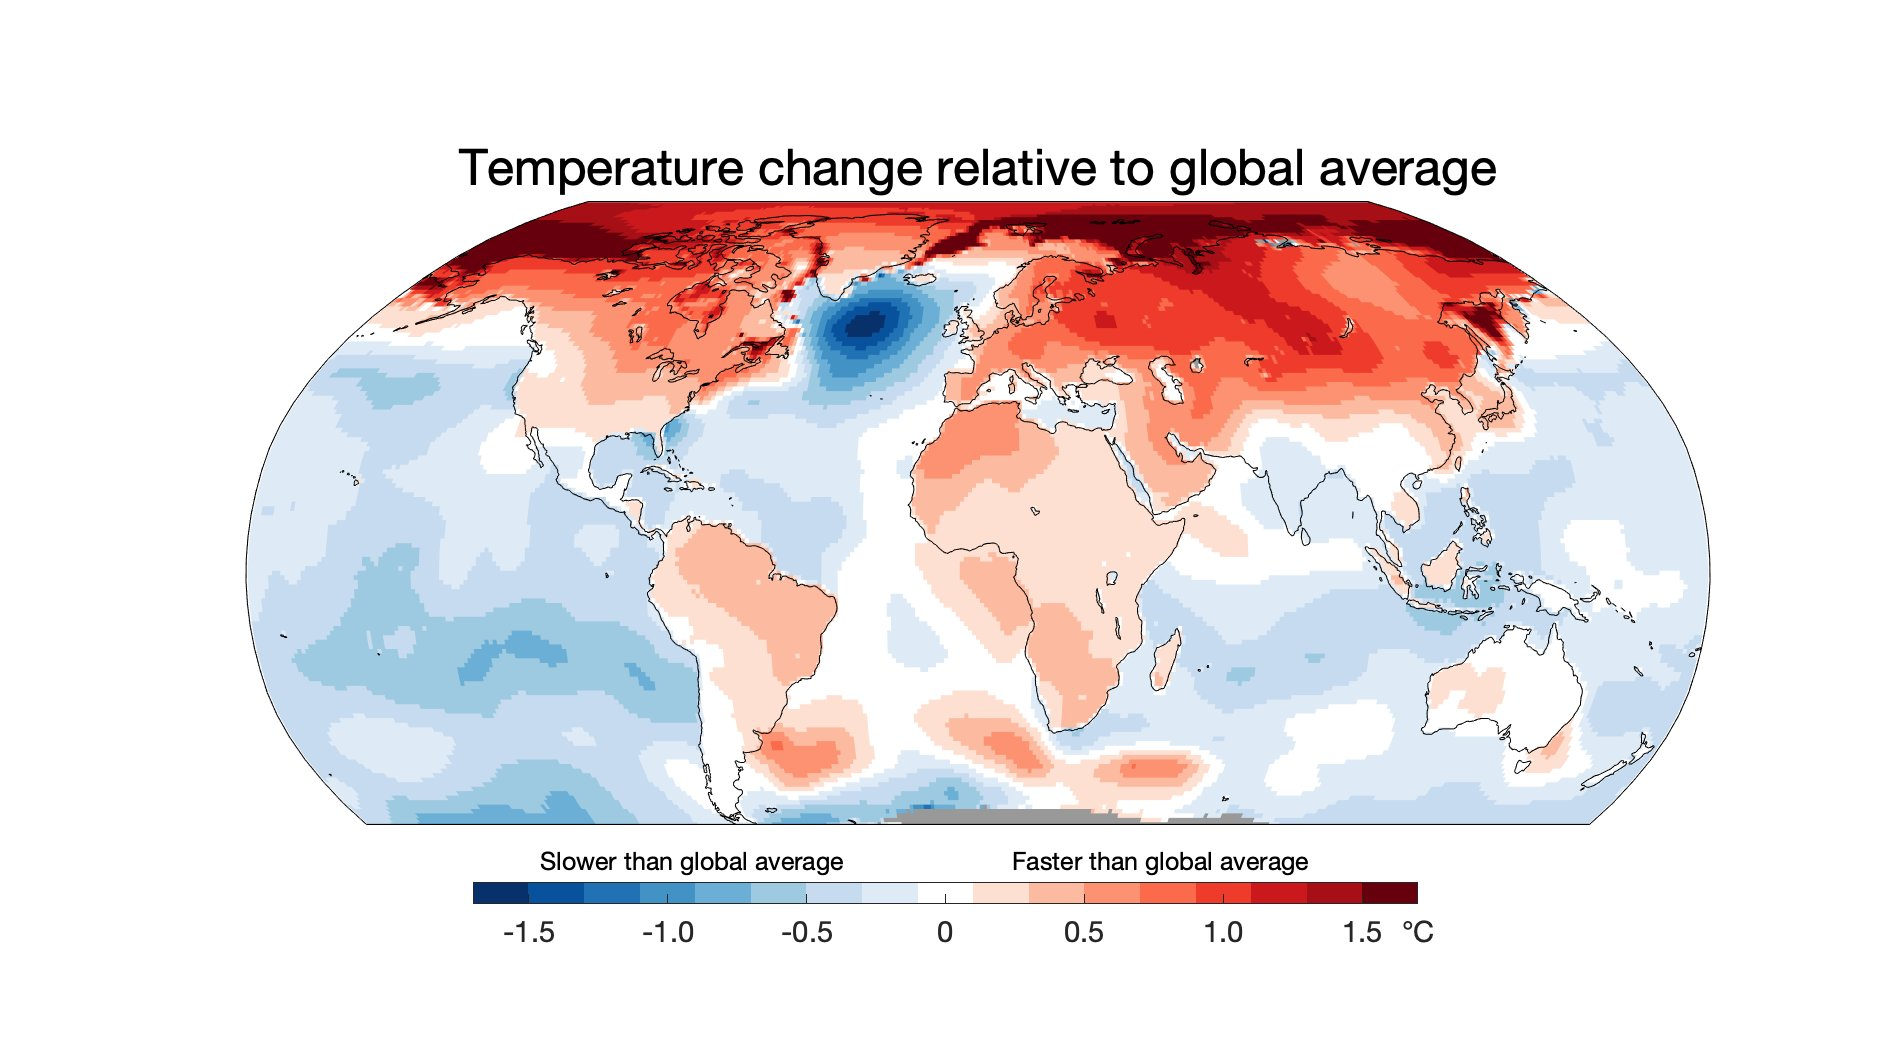
\includegraphics{fig/World_Temp_Change_Speed.jpeg}

\hypertarget{part-elements}{%
\part{Elements}\label{part-elements}}

\hypertarget{albedo}{%
\chapter{Albedo}\label{albedo}}

Some text on Albedo

\hypertarget{atmosphere}{%
\chapter{Atmosphere}\label{atmosphere}}

\begin{verbatim}
- Emissions
    - CO2    
    - Methane
    -
- Attributing Emissions
    - Norway's Responsibility
\end{verbatim}

\hypertarget{emissions}{%
\section{Emissions}\label{emissions}}

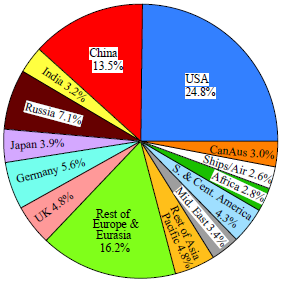
\includegraphics{fig/Emissions_Sum_1751-2018_by_Region.png}

Fig: Cumulative Emissions 1751-2018 by Country/Region

The UK (like the US) is 5X more responsible for global warming than the average nation.

\hypertarget{co2}{%
\subsection{CO2}\label{co2}}

\hypertarget{methane}{%
\subsection{Methane}\label{methane}}

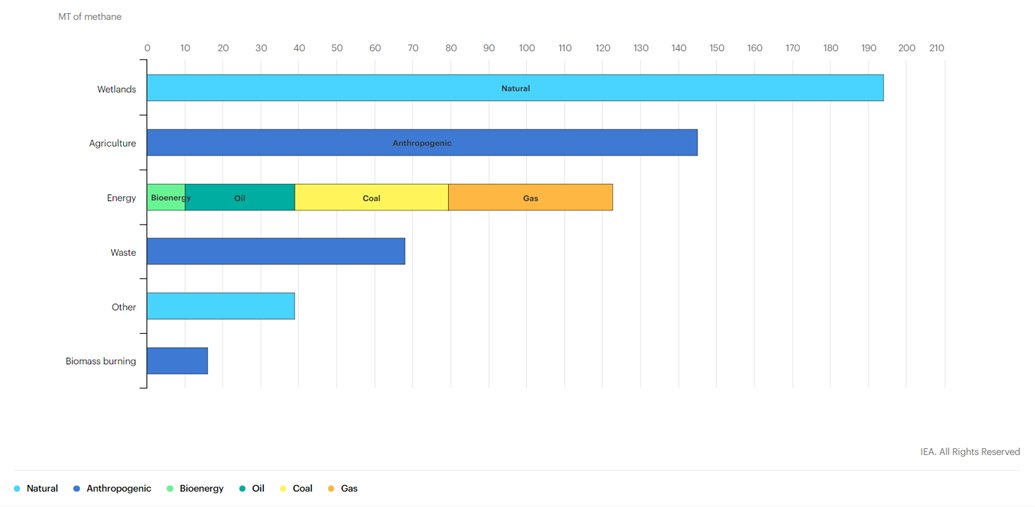
\includegraphics{fig/Methane_by_Source.jpeg}

Methane, the largest component of natural gas, is sometimes called a ``short-lived climate pollutant'' because it remains in the atmosphere for far less time than carbon dioxide, which can remain in the atmosphere for hundreds of years. But methane is also a climate ``super-pollutant,'' 86 times more potent than carbon dioxide at warming the atmosphere over a 20-year period.

Sources of methane include wetlands, rice paddies, livestock, biomass burning, organic waste decomposition and fossil fuel drilling and transport.

\hypertarget{cut-methane-now}{%
\subsubsection{Cut Methane Now}\label{cut-methane-now}}

Methane is the biggest and really the only lever we have to slow
temperature rise during the next two decades.

Methane's potency and short atmospheric life make it a key greenhouse gas for policy makers to focus on as a way to combat global warming in the near term because the impact of those cuts will be felt almost immediately.

``If we cut methane emissions substantially during the 2020s, the abundance or concentration in the atmosphere will also drop rapidly during the 2020s,'' said Drew Shindell, an earth science professor at Duke University. ``If we cut CO2 emissions, it takes a long time for actual concentrations to drop, and then longer for the climate to adjust.''

\href{https://insideclimatenews.org/news/20042021/methane-biden-climate-summit/}{Inside}

\hypertarget{attributing-emissions}{%
\section{Attributing Emissions}\label{attributing-emissions}}

\hypertarget{norways-responsibility}{%
\subsection{Norway's Responsibility}\label{norways-responsibility}}

\begin{verbatim}
In real life responsibility is more than what is legally binding
\end{verbatim}

The emissions of CO2 that occur within Norway's territory are dwarfed by the emissions that result from combustion of all the oil and gas Norway produces. Because these fossil fuels are exported before being combusted, the emissions are allocated to the accounts of other countries. If Norway had generated electricity from the gas and then exported the electricity, for example, then emissions from that electricity generation would be allocated to Norway's accounts. There is therefore an element of artificiality associated with this allocation. It takes two to tango.

Norway's territorial emissions of CO2 were about 42 Mt in 2019, and over 1971--2019 totalled about 1.9 Gt. In comparison, emissions from Norwegian oil and gas since 1971 have been about 16 Gt. A similar amount (\textasciitilde15 Gt) will be emitted if all remaining Norwegian oil and gas resources are extracted from the continental shelf.

In 2019, emissions from Norwegian oil and gas amounted to 84 tonnes of CO2 for every person in Norway.

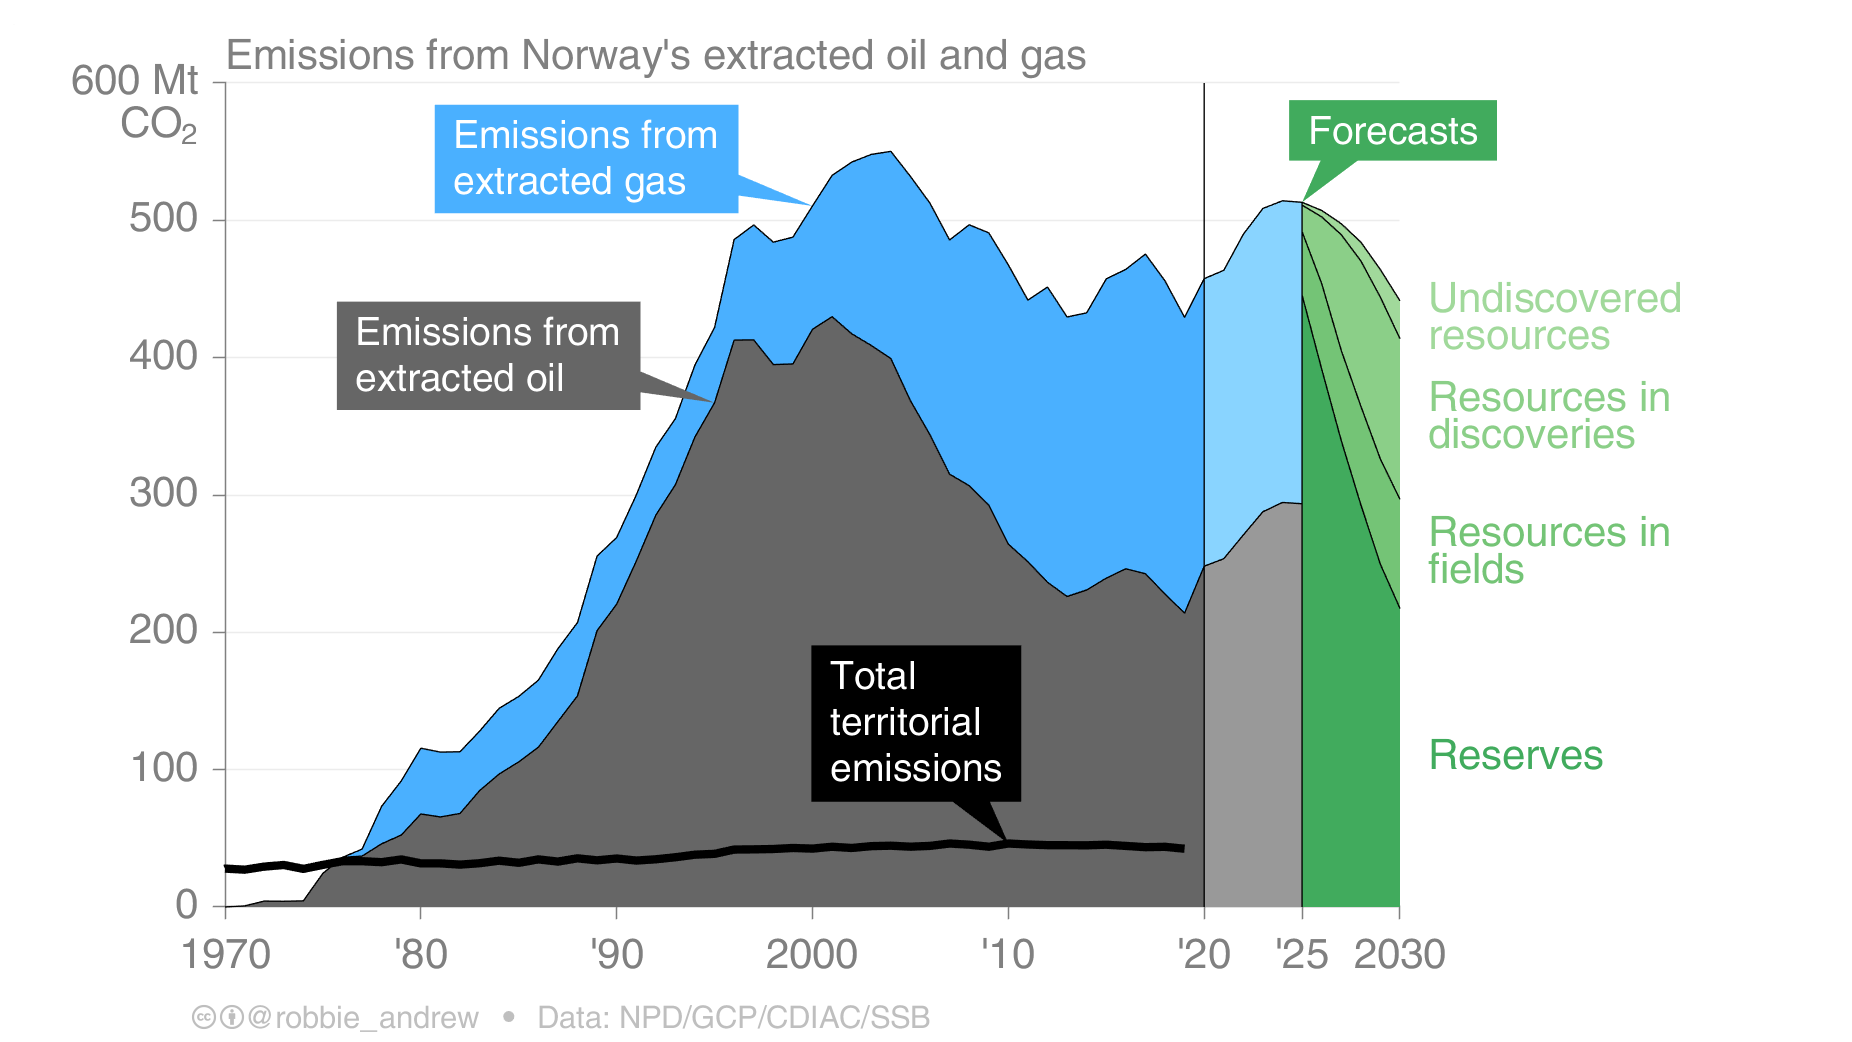
\includegraphics{fig/Emissions_extracted_Oil_Gas_Norway.png}

\href{https://folk.universitetetioslo.no/roberan/t/export_emissions.shtml}{Norways Export Emissions (Robbie Andrew)}

In Norwegian politics, there's been a very successful attempt to separate the discussion of oil policy from the discussion of climate policy. The two were never really tightly linked {[}in the country{]} until roughly the last decade, and this division has become increasingly difficult to maintain.

Norwegian politicians also haven't been alone in creating the conditions that made this division possible. They've been helped immensely by the international climate regime.

From the very beginning of international climate policy, there was this agreement that countries had to account for the emissions that they create when they burn fossil fuels. All the responsibility was placed on the demand side, not the supply side, which was very convenient for Norway.

Europe is the primary market for Norway's oil and gas. But determining the climate effects of Norwegian production is not straightforward. One study has estimated a clear climate benefit from reducing oil output, but the market is complex and the result really depends on your assumptions about how other actors will behave and how the market will evolve over time.

The big irony here is that Norway is a fairly large fossil-fuel producer, but we use relatively few fossil fuels directly in our energy use. Nearly all of our electricity has for a long time come from hydropower. In most years, we even export quite a lot of renewable electricity to our neighbors.
The only place where fossil fuels are used to directly produce energy is to run the platforms offshore. They use gas to run the turbines to get the energy needed for oil and gas production.

The government's new climate plan, which was unveiled just a few days ago, does include a number of new and more aggressive measures to reduce Norway's domestic emissions. The proposal to increase the already quite high CO2 tax on offshore emissions came as something of a surprise, and it is likely to pass even if it is currently being challenged by the industry.

However, it is important to keep in mind that this proposal only targets the production-related emissions of Norwegian oil, not the level of oil that is being extracted and exported. As such, it is in line with the historical separation between climate and oil policymaking, which tends to focus only on emissions happening within Norway and exclude any concern for the climate impact of exported oil and gas.

The Norwegian paradox has worked out fairly well up until the last few years because there has been little focus on the production of fossil fuels, and because Norway is small enough to avoid the scrutiny that some larger nations face. But this is quickly changing, both in the domestic and international political discussion.

There is now a lot more focus on the supply side of fossil fuels than 10 years ago, with several countries like Denmark announcing an end to drilling and new research showing a mismatch between planned fossil-fuel production and ideas such as a ``non-proliferation treaty'' for fossil fuels being floated. The treaty would bring the world together in agreeing to end the use of fossil fuels much like the UN came together to curb the spread of nuclear weapons.

This will make it increasingly hard for Norway to hold on to a leadership claim as long as oil production keeps being expanded into new areas.

\href{https://www.vox.com/22227063/norway-oil-gas-climate-change}{Norways Climate - Petroleum Dilemma (Bard Lahn)}

\hypertarget{global-north-vs-south-responsibility}{%
\subsection{Global North vs South Responsibility}\label{global-north-vs-south-responsibility}}

The global North is responsible for 92\% of total excess carbon dioxide emissions.
Climate breakdown is colonial in character and ultimately requires an anti-colonial struggle in response. (Jason Hickel)

\begin{figure}
\centering
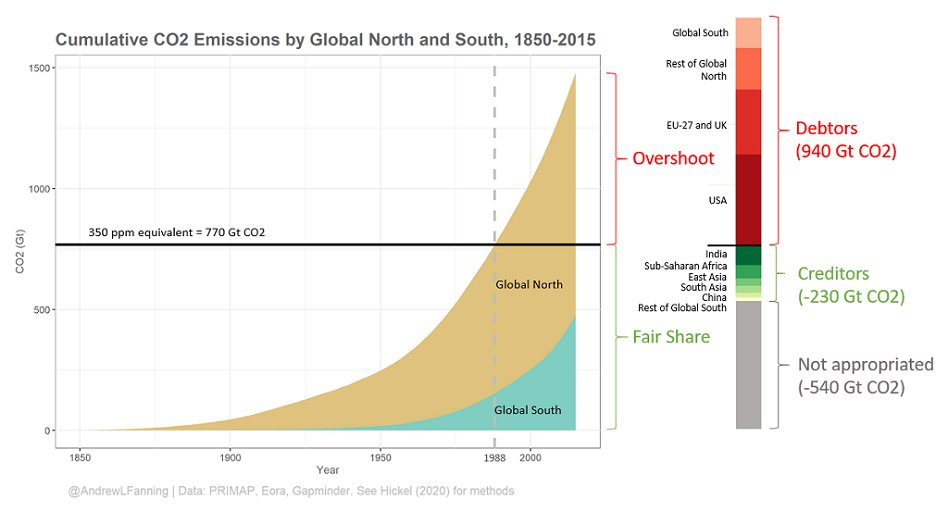
\includegraphics{fig/CO2_Emissions_Global_North_South.jpeg}
\caption{Fig. by \citet{AndrewFanning}}
\end{figure}

\hypertarget{forests}{%
\chapter{Forests}\label{forests}}

\hypertarget{forests-tipping-go-from-sink-to-source-of-co2-due-to-temperature-increase.}{%
\section{Forests tipping: go from sink to source of CO2 due to temperature increase.}\label{forests-tipping-go-from-sink-to-source-of-co2-due-to-temperature-increase.}}

New research shows that Earth's overheated climate will
alter forests at a global scale even more fundamentally,
by flipping a critical greenhouse gas switch in the next few decades.
The study suggests that, by 2040, forests will take up only
half as much carbon dioxide from the atmosphere as they do now,
if global temperatures keep rising at the present pace.

Global warming has contributed to thinning canopies in European forests
and to sudden die-offs of aspen trees in Colorado,
as well as insect outbreaks that are killing trees around the world.
In many places, forests are not growing back.

The data show a clear temperature limit,
above which trees start to exhale more CO2 than they can take in through photosynthesis.
The findings mark a tipping point, of sorts, at which ``the land system will act to accelerate climate change rather than slow it down,''

\href{https://insideclimatenews.org/news/13012021/forests-heat-climate-change/}{Trees From Sink to Source (InsideClimateNews)}

At present, the land provides a ``climate service'' by absorbing
around 30 per cent of the emissions caused by humans each year.

Unlike other tipping elements in the Earth system, the climate tipping point
for the terrestrial biosphere could be exceptionally close --
20-30 years away -- without action.

Plant respiration, the process by which plants produce energy for growth,
causes CO2 to be released into the atmosphere.

The `buffer' or `discount' against carbon emissions that we currently receive from the biosphere is more fragile than we previously realised.

Climate models are tools used by scientists to simulate how the world is likely to respond to greenhouse gas emissions.

However, it is worth noting that the global dataset used in the study
uses ``very few samples from tropical regions''.
This means that it is still not fully understood how tropical forests
are responding to rising temperatures.

\href{https://www.independent.co.uk/environment/climate-change/land-ecosystems-tipping-point-temperature-b1786822.html}{Independent}

\emph{Memo Duffy}

The temperature dependence of global photosynthesis and respiration
determine land carbon sink strength.
While the land sink currently mitigates \textasciitilde30\% of anthropogenic carbon emissions,
it is unclear whether this ecosystem service will persist and
what hard temperature limits, if any, regulate carbon uptake.

The mean temperature of the warmest quarter (3-month period)
passed the thermal maximum for photosynthesis during the past decade.
At higher temperatures, respiration rates continue to rise
in contrast to sharply declining rates of photosynthesis.

Under business-as-usual emissions, this divergence elicits a
near halving of the land sink strength by as early as 2040.

The difference between gross primary productivity
and total ecosystem respiration
(carbon uptake by vegetation minus carbon loss to the atmosphere)
comprises the metabolic component of the land carbon
sink {[}net ecosystem productivity (NEP){]}.

To date, land ecosystems provide a climate regulation service
by absorbing \textasciitilde30\% of anthropogenic emissions annually.
While temperature functions as a key driver
of year-to-year changes in the land carbon sink,
its temperature response is still poorly constrained at biome to global scales,
making the carbon consequences of anticipated warming uncertain.

Like all biological processes, metabolic rates for photosynthesis
and respiration are temperature dependent; they accelerate with in-
creasing temperature, reach a maximum rate, and decline thereafter.

Highly divergent land carbon sink trajectories from Earth system models.

Continued future increases in sink strength due to the CO2 fertilization.

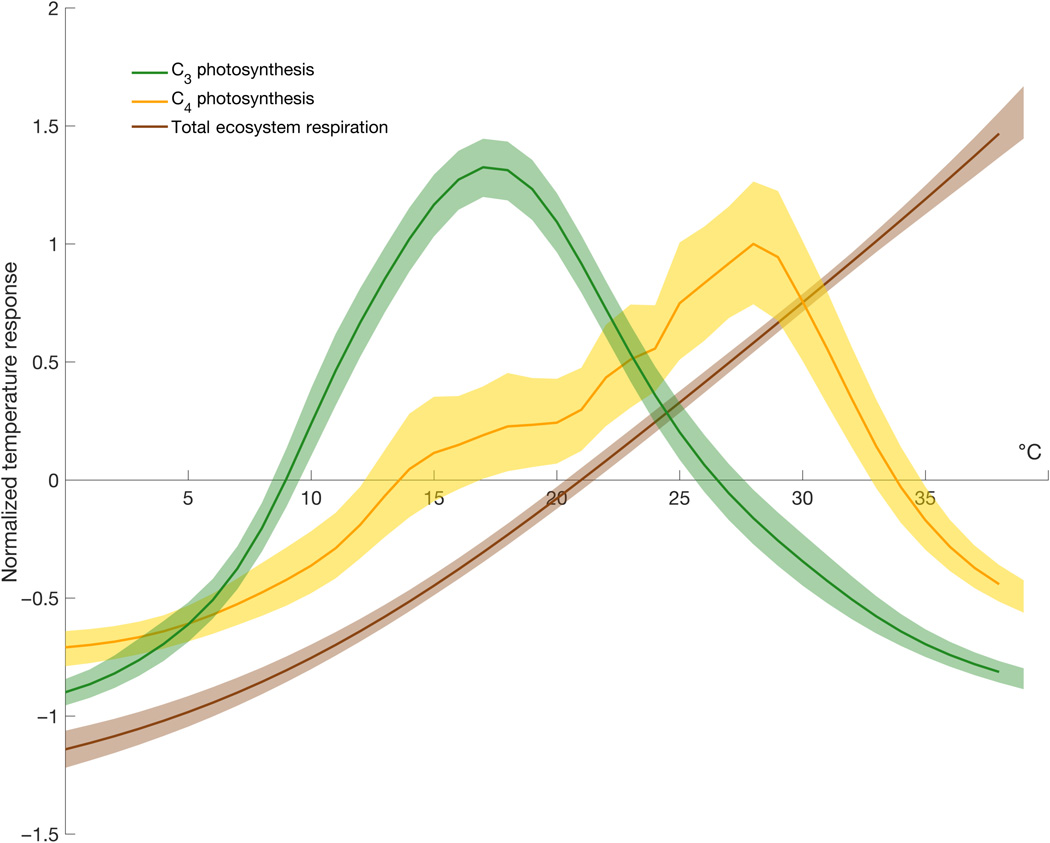
\includegraphics{fig/Photosythesis_Temp_Response.jpg}

The temperature response of global photosynthesis
shows distinct maxima at 18°C for C3 and 28°C for C4 plant systems.
In contrast to photosynthesis, respiration rates increase across
the range of ambient temperatures (up to 38°C),
with no evidence of Tmax or rate decline.
The thermal maxima of leaf and soil respiration reside at \textasciitilde60°-70°C.

Responses diverge at temperatures above Tmax.
The imbalance grows more pronounced as temperature increases.

Current climate mostly lies just below Tmax where slight increases in temperature act as
climate fertilization of land carbon uptake.
Under anticipated warming foreshadowed by historical temperature extremes and coincident
land carbon loss---however, more and more time will be spent above Tmax.
Past this threshold, the land carbon balance will first weaken and
ultimately reverse sign from carbon sink to carbon source.

25°C constitutes a powerful tipping point for the land
sink of carbon and a formidable positive climatic feedback,

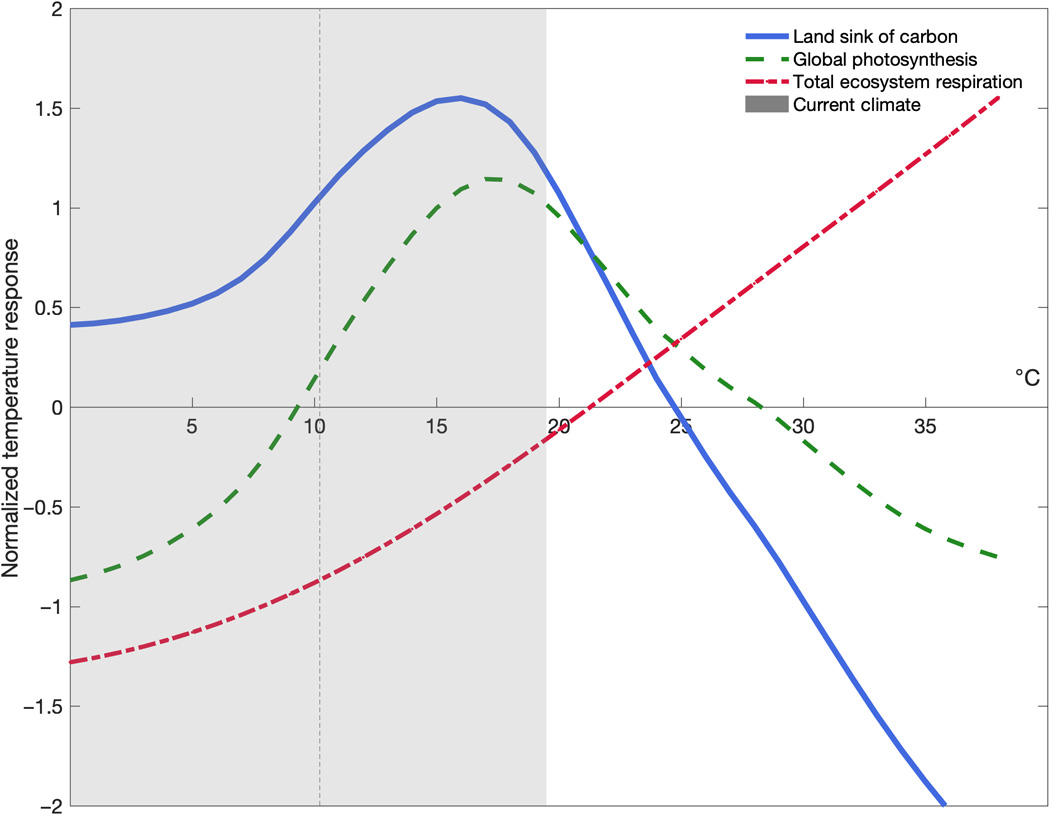
\includegraphics{fig/Land_Sink_of_Carbon.jpg}

Currently, less than 10\% of the terrestrial biosphere experiences
where land carbon uptake is degraded.
For regions that do experience these temperatures,
exposure is limited to 1 to 2 months or
constitutes areas with sparse to no vegetation.

Under business-as-usual emissions, by 2100, up to half
of the terrestrial biosphere could experience temperatures past
the treshold.

The impact of elevated temperatures on the land sink is more than a
function of cumulative area.
Biomes that cycle 40 to 70\% of all terrestrial carbon
including the rainforests of the Amazon and Southeast Asia and
the Taiga forests of Russia and Canada
are some of the first to exceed biome-specific Tmax
for half the year or more.
This reduction in land sink strength is effectively front-loaded
in that a 45\% loss occurs by midcentury,
with only an additional 5\% loss by the end of the century.
These estimates are conservative as they assume
full recovery of vegetation after temperature stress and
ignore patterns and lags in recovery.

In contrast to any CO2 fertilization effect,
anticipated higher temperatures associated with
elevated CO2 could degrade land carbon uptake.
Failure to account for this results in
a gross overestimation of climate change mitigation provided by terrestrial vegetation.

We are rapidly entering temperature regimes where biosphere productivity
will precipitously decline and
calls into question the future viability of the land sink.

\href{https://advances.sciencemag.org/content/7/3/eaay1052}{Duffy(2021) Temperature tipping point of the terrestrial biosphere}
\href{pdf/Duffy_2020_Temperature_Tipping_Point.pdf}{(pdf)}

\hypertarget{plant-and-cut---forest-ccs}{%
\section{Plant and Cut - Forest CCS}\label{plant-and-cut---forest-ccs}}

Wood can also serve purely as a long-term carbon storage device. The key to locking away the carbon is to cut off the oxygen supply to microbes, thereby preventing decomposition.

Natural experiments show how this can be done. 19th-century lumberjacks in the US and Canada frequently stored logs on the surfaces of the Great Lakes or floated them down rivers, some of which ended up sinking along the way. These have remained in such good condition that a modern-day cottage industry has arisen to recover the logs and turn them into everything from hardwood floors to violins. New Zealand has a similar industry with logs that were fortuitously buried in swamps as long as 60,000 years ago.

Based on such examples, scholars have proposed chopping down trees or collecting fallen logs and intentionally stowing them away. That could mean sinking them to the bottom of lakes, interring them in abandoned mines or burying them in specially dug trenches.
The idea hasn't gotten much traction yet, but in 2013, the Quebec Ministry of Agriculture, Fisheries and Food funded a pilot project to dig a trench and bury 35 metric tons of wood. The project came to about \$29 per metric ton of CO2 sequestered, according to government scientist Ghislain Poisson, in line with a theoretical estimate of \$10-\$50.

That is cheaper than most high-tech forms of carbon capture and storage, which usually involve machines that filter carbon out of the air and pump it underground. Sequestering carbon at the typical power plant, where emissions are highly concentrated, runs to \$30-\$91 per metric ton of CO2, but in open air, which is the holy grail, costs theoretically range from \$94-\$232. To help this promising new technology get off the ground (or rather, into the ground), the federal government offers a tax credit of about \$35 for every metric ton of CO2 removed in industrial carbon capture and storage. It's a policy that has enjoyed strong bipartisan support for over a decade.

\href{https://edition.cnn.com/2021/02/10/opinions/climate-plant-and-cut-trees-down-bader/index.html}{Plant and Cut (CNN)}

\hypertarget{deforestation-footprint}{%
\section{Deforestation Footprint}\label{deforestation-footprint}}

(see: env)

\href{Nature,\%20paywall}{Hoang: Mapping Deforestation Footprint}{]}(\url{https://www.nature.com/articles/s41559-021-01417-z})

\hypertarget{ice-sheet}{%
\chapter{Ice Sheet}\label{ice-sheet}}

\hypertarget{greenland}{%
\section{Greenland}\label{greenland}}

\emph{Abstract Noel}

Under anticipated future warming, the Greenland ice sheet (GrIS) will
pass a threshold when meltwater runoff exceeds the accumulation of snow,
resulting in a negative surface mass balance (SMB \textless{} 0) and sustained mass loss.

Here we dynamically and statistically downscale the outputs of an
Earth system model to 1 km resolution to infer that a Greenland near‐surface
atmospheric warming of 4.5 ± 0.3 °C---relative to pre‐industrial---is required
for GrIS SMB to become persistently negative.

Climate models from CMIP5 and CMIP6 translate this regional temperature change
to a global warming threshold of 2.7 ± 0.2 °C.
Under a high‐end warming scenario, this threshold may be reached around 2055,
while for a strong mitigation scenario it will likely not be passed.
Depending on the emissions scenario taken, our method estimates a 6‐13 cm sea level rise
from GrIS SMB in the year 2100.

\href{https://agupubs.onlinelibrary.wiley.com/doi/10.1029/2020GL090471}{Noel (2021) Greenland Ice Sheet Loss}
\href{pdf/Noel_2021_Greenland_Ice_Sheet_Loss.pdf}{(pdf)}

\hypertarget{antarctica}{%
\section{Antarctica}\label{antarctica}}

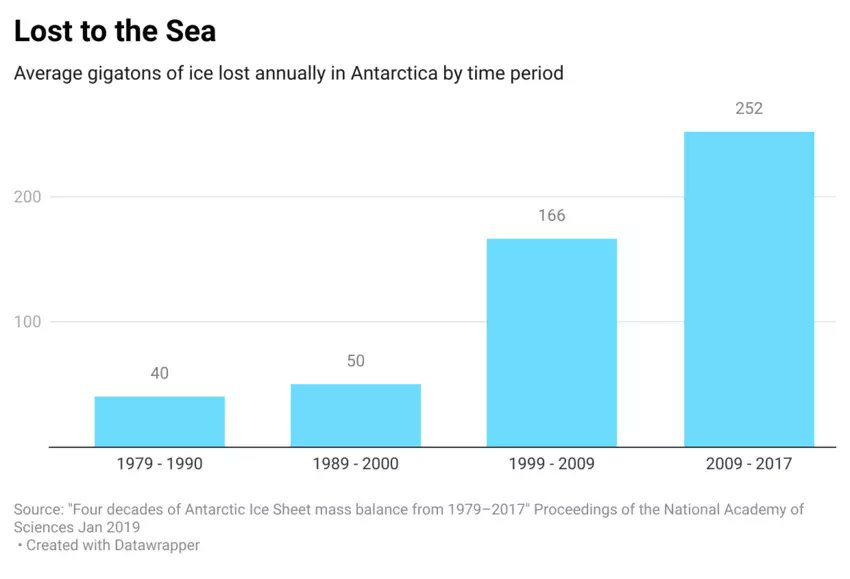
\includegraphics{fig/Antarctica_Ice_Loss_to_Sea.jpeg}

\hypertarget{ocean}{%
\chapter{Ocean}\label{ocean}}

\hypertarget{sea-level-rise}{%
\section{Sea Level Rise}\label{sea-level-rise}}

In its most recent assessment, the Intergovernmental Panel on Climate Change said the sea level was unlikely to rise beyond 1.1 metre (3.6ft) by 2100.

But climate researchers from the University of Copenhagen's Niels Bohr Institute believe levels could rise as much as 1.35 metres by 2100, under a worst-case warming scenario.

``The models used to base predictions of sea level rise on presently are not sensitive enough,'' he said. ``To put it plainly, they don't hit the mark when we compare them to the rate of sea level rise we see when comparing future scenarios with observations going back in time.''

\href{https://www.theguardian.com/environment/2021/feb/02/sea-level-rise-could-be-worse-than-feared-warn-researchers}{Higher Sea Level Rise (Guardian)}

\hypertarget{tsls-transient-sea-level-sensitivity}{%
\subsection{TSLS Transient Sea Level Sensitivity}\label{tsls-transient-sea-level-sensitivity}}

By analyzing the mean rate of change in sea
level (not sea level itself), we identify a nearly linear rela-
tionship with global mean surface temperature (and there-
fore accumulated carbon dioxide emissions) both in model
projections and in observations on a century scale. This mo-
tivates us to define the ``transient sea level sensitivity'' as the
increase in the sea level rate associated with a given warm-
ing in units of meters per century per kelvin. We find that
future projections estimated on climate model responses fall
below extrapolation based on recent observational records.
This comparison suggests that the likely upper level of sea
level projections in recent IPCC reports would be too low.

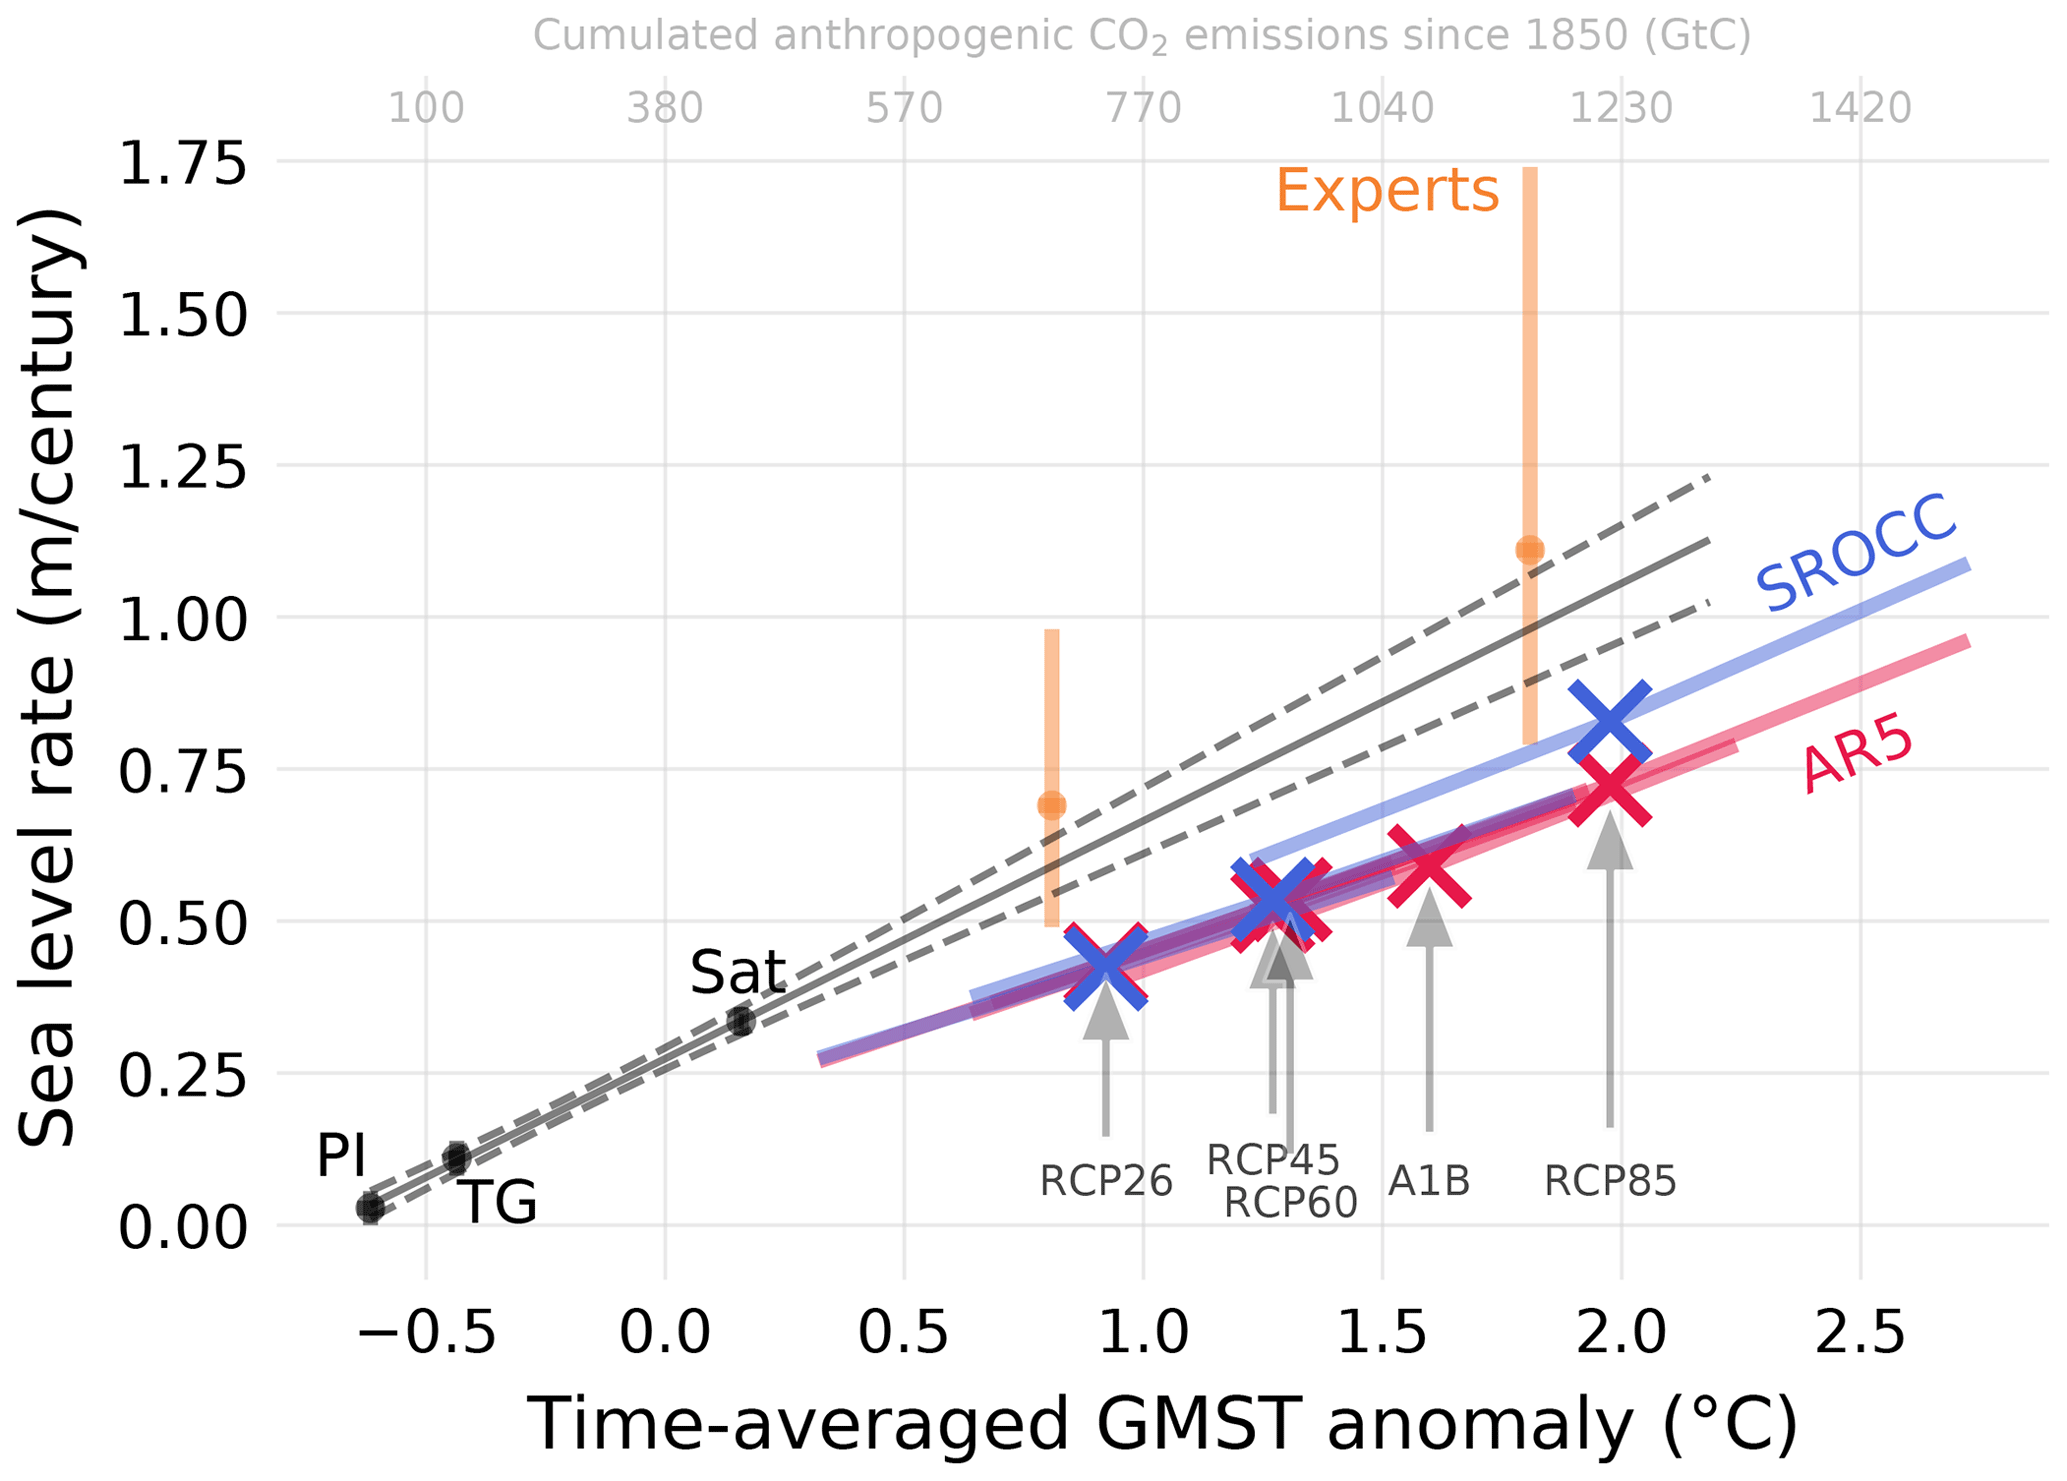
\includegraphics{fig/Transient_Sea_Level_Sensitivity.png}

Sea level projections as assessed in AR5 and SROCC systematically fall
below what would be expected from extrapolating observations to
warmer conditions, as well as below the expert elicitation. Error
bars show estimated likely ranges (17 \%--83 \%).

\href{https://os.copernicus.org/articles/17/181/2021/}{Grindsted (2021) Transient Sensitivity of Sea Level Rise (Ocean Science)}
\href{pdf/Grindsted_2021_Transient_Sensitivity_of_Sea_Level_Rise.pdf}{(pdf)}

\hypertarget{amoc---gulf-stream}{%
\section{AMOC - Gulf Stream}\label{amoc---gulf-stream}}

\textbf{Weakest Gulf Stream in Millenium}

The Atlantic Meridional Overturning Circulation (AMOC)---one of Earth's major ocean circulation systems---redistributes heat on our planet and has a major impact on climate. Here, we compare a variety of published proxy records to reconstruct the evolution of the AMOC since about ad 400. A fairly consistent picture of the AMOC emerges: after a long and relatively stable period, there was an initial weakening starting in the nineteenth century, followed by a second, more rapid, decline in the mid-twentieth century, leading to the weakest state of the AMOC occurring in recent decades.

\href{https://www.nature.com/articles/s41561-021-00699-z}{Caesar (2021) AMOC Millenium Weakest (Nature Geoscience) {[}paywall!{]}}

\href{https://twitter.com/rahmstorf/status/1364976597250568194}{Rahmstorf - Twitter Thread}

\href{https://www.theguardian.com/environment/2021/feb/25/atlantic-ocean-circulation-at-weakest-in-a-millennium-say-scientists}{The Guardian}

\href{https://www.theguardian.com/commentisfree/2021/feb/26/atlantic-currents-climate-oceans-next-century}{The Guardian (Commentary)}

\hypertarget{the-rise-and-fall-of-amoc}{%
\subsection{The Rise and Fall of AMOC}\label{the-rise-and-fall-of-amoc}}

The AMO is simply an artifact of studies that misinterpret
the time-varying pattern of human-caused climate change
as a low-frequency oscillation

At times I feel like I created a monster when I gave a name to this putative climate oscillation in 2000. The concept of the AMO has since been misapplied and misrepresented to explain away just about every climate trend under the sun, often based on flawed statistical methods that don't properly distinguish a true climate oscillation from a time-varying trend: If you assume that all trends are a simple linear ramp, and call everything left-over an ``oscillation'', then the simple fact that global warming flattened out from the 1950s through the 1970s driven by the ramp-up in cooling sulphate aerosol pollution masquerades as an apparent ``oscillation'' on top of a simple linear trend. We've published a number of articles over the years (see e.g.~here, here, here, here, here, and here) demonstrating that studies that use such an approach to define the AMO end up mis-attributing to a natural ``oscillation'' what is actually human-caused climate change. Such analyses have been used by some to dismiss, among other things, the impact climate change is having on increasingly active and destructive Atlantic hurricane seasons, attributing the increase in recent decades to a supposed upturn in the AMO.

\href{http://www.realclimate.org/index.php/archives/2021/03/the-rise-and-fall-of-the-atlantic-multidecadal-oscillation/}{RealClimate}

\hypertarget{rethinking-amoc}{%
\subsection{Rethinking AMOC}\label{rethinking-amoc}}

\emph{Chafik}

A weakened AMOC may have played a role in causing almost 600 years' worth of frigid winters in Europe and North America. This period, called the Little Ice Age, lasted roughly from 1300 until 1870 and came on the heels of the Medieval Warm Period (circa 950--1250), when temperatures in the Northern Hemisphere were unusually warm.

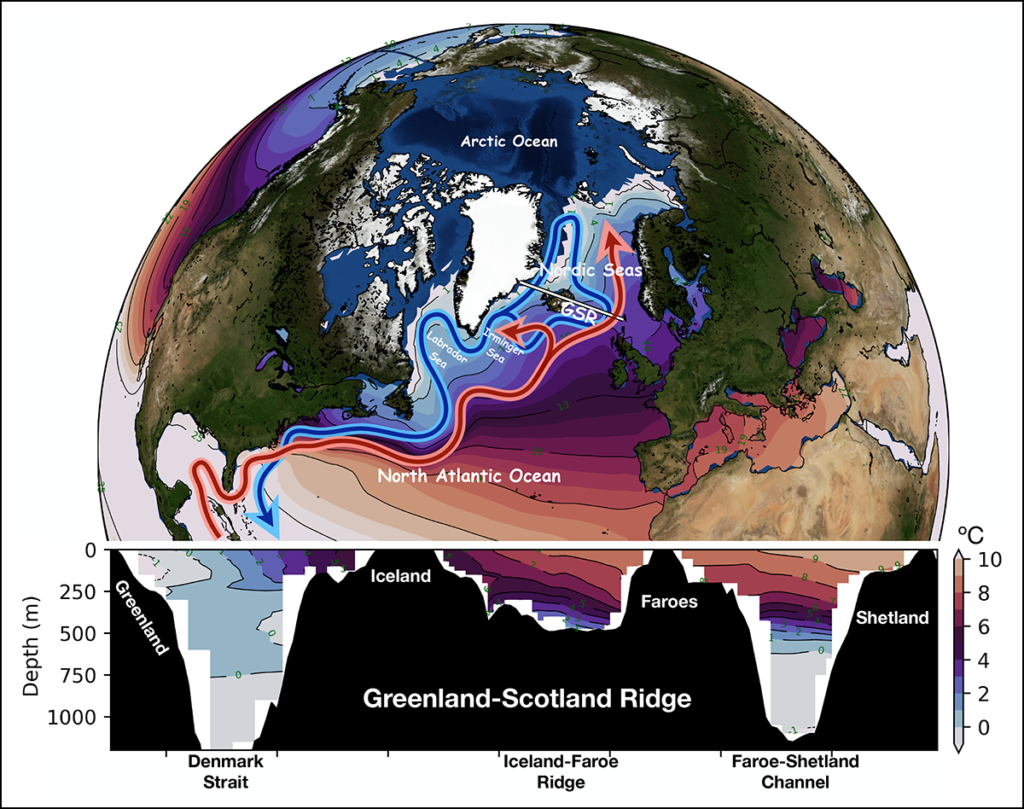
\includegraphics{fig/surface-deep-circulation-north-atlantic.png}

\emph{Figure: This simplified view (top) shows the surface flows (red arrows) and deep return flows (blue arrows) that make up the large-scale ocean circulation in the North Atlantic. Color bands on the ocean surface indicate average sea surface temperatures from 1900 to 2019 (data are from the Hadley Centre) and highlight the northward extent of warm waters to higher latitudes. The longitude-depth temperature distribution of the ocean (bottom; data are from the World Ocean Atlas 2018) across the Greenland-Scotland Ridge (GSR, white transect line in the top panel) is also shown. The exchange of waters across the GSR is driven by the rapid loss of heat to the atmosphere over the Nordic Seas. This heat loss causes the waters to sink and build a huge reservoir of cold, dense water that spills back into the deep North Atlantic across the GSR, completing the overturning process.}

Nearly half of the AMOC's poleward flow of warm, salty waters enters the Nordic Seas---comprising the Greenland, Iceland, and Norwegian Seas. Here the water cools and pools north of the undersea Greenland-Scotland Ridge (GSR).
A host of important questions remains about the dynamics of the ocean near the GSR and the effects of these dynamics on regulating climate.

The AMOC has two pathways of overturning circulation. One is open ocean convection in the Irminger and Labrador Seas that produces the upper layer of North Atlantic Deep Water (NADW).
The second involves progressive cooling of warm, salty water from the Atlantic in the Nordic Seas. This cooling results in dense water spilling over the GSR back into the North Atlantic---mainly through two passages, the Denmark Strait between Greenland and Iceland and the Faroe Bank Channel south of the Faroes---and forming a lower layer of NADW.

Both regions depend upon heat loss to produce water of greater density, but it appears that huge heat losses from the Nordic Seas and the concomitant production and pooling of very dense water behind the GSR are fundamental to maintaining a mild climate in northern Europe. This heat loss produces a healthy supply of NADW that spills back into the global abyss and enables warm, salty water to feed the Nordic Seas.

Evidence of strong variability in Nordic Seas inflow on multidecadal timescales.
The volume of and heat transported in this poleward flow, as measured at the GSR, are strongly coupled to the Atlantic multidecadal variability (AMV), which describes natural patterns of sea surface temperature variability in the North Atlantic that influence climate globally

The AMV affects Nordic Seas inflow because deep convection in the northeast Atlantic translates the surface temperature variations down into the upper layers of the ocean, and these variations shape the ocean's dynamic height field.

The inflow of warm water to the Nordic Seas has been quite stable over the past century since the start of modern oceanography.

Nordic Seas overturning circulation has been stable over the past 100 years. This stability is surprising given the extraordinary warming presently underway in the Nordic Seas and Arctic Ocean.
The continued stability of this vital ocean circulation system is not guaranteed in the future. It is also unclear how future change may manifest or which early-warning indicators should be relied upon to forecast change.

The recent discovery of an unknown route by which cold water courses its way through the Norwegian Sea. We identified that this new route directs cold deep flows north of the Faroe Islands to the Norwegian slope before turning them south through the Faroe-Shetland Channel and into the deep North Atlantic.

Which route water takes north of the GSR and how much is funneled each way depend on the prevailing winds.

Under weak westerly wind conditions in the Nordic Seas, the densest water that feeds the Faroe Bank Channel comes primarily from north of Iceland. During strong westerly wind conditions, however, more water seems to originate from along the Jan Mayen Ridge, which is located farther north of Iceland and more in the middle of the Nordic Seas. This wind dependence is curious, considering the strong control that bathymetry can exert on the circulation.

Deep rapid flow, or deep jet, called the Faroe-Shetland Channel Jet. Remarkably, this jet flows south along the eastern slope of the channel rather than along the western side as has long been assumed. The deep jet is found to be the main current branch in terms of transport that delivers the densest water to the North Atlantic Ocean via the Faroe Bank Channel. This surprising finding countered past observations and thinking.

We do not yet have a firm grasp of the deep circulation of the Nordic Seas and how it varies over time.

All available observational evidence so far indicates that there is no long-term trend in the Nordic Seas meridional overturning circulation to date.

The degree to which fresh water from the Arctic and Greenland Sea can mix with and dilute warm, saline water from the Atlantic. Such dilution could suppress deep temperature- and density-driven convection, thus weakening or shutting down the overturning in the Nordic Seas and, by extension, the deepest component of the AMOC.

However, most scientists \href{https://www.carbonbrief.org/guest-post-could-the-atlantic-overturning-circulation-shut-down}{no longer think} such a shutdown scenario is likely because observations to date indicate that Arctic and Greenland waters tend to remain trapped around and south of Greenland rather than mixing and diluting the Atlantic water flowing north in the Nordic Seas

Nonetheless, there is broad agreement that the climatic consequences of a potential shutdown of this vital ocean circulation are so enormous that they obligate us to improve our understanding of the Nordic Seas.

\href{https://eos.org/science-updates/rethinking-oceanic-overturning-in-the-nordic-seas\#.YHvKO1RSYTk.twitter}{Chafik (2021) Rethinking Oceanic Overturning in Nordic Seas}

\hypertarget{permafrost}{%
\chapter{Permafrost}\label{permafrost}}

Some text on Permafrost

\hypertarget{soil}{%
\chapter{Soil}\label{soil}}

\emph{Guardian}

The storage potential of one of the Earth's biggest carbon sinks -- soils -- may have been overestimated, research shows. This could mean ecosystems on land soaking up less of humanity's emissions than expected, and more rapid global heating.

The study, based on over 100 experiments, found the opposite. When plant growth increases, soil carbon does not. The finding is significant because the amount of organic carbon stored in soils is about three times that in living plants and double that in the atmosphere. Soils can also store carbon for centuries, whereas plants and trees rot quickly after they die.

When rising CO2 increases plant growth, there is a decrease in soil carbon storage.
If soils do absorb less in future, ``the speed of global warming could be higher''

Soils, plants and trees are important for carbon levels,
but ending the burning of fossil fuels is essential.
To stop global warming, we need to stop emissions,
because ecosystems only take up a fraction of all the CO2 emissions.

The researchers found that in grasslands, elevated CO2 led to 9\% plant growth -- less than forests -- but soil carbon rose by 8\%. Terrier said there has been a lot of discussion about tree planting as a way to tackle the climate crisis. ``What I found very concerning in that debate is that people were suggesting planting trees in natural grasslands, savannah, and tundra,'' he said. ``I think that would be a terrible mistake because, as our results imply, there is a very large potential to increase soil carbon storage in grasslands.''

Given that the land absorbs 30\% of the carbon emitted from fossil fuels and deforestation, understanding if that will change in the future matters.
Change would be determined by the balance between rising CO2 boosting plant growth and the negative effects of climate change itself, including drought, heatwaves and fires. The evidence to date suggests the biggest change will be the negative effects of global heating on ecosystems

\href{https://www.theguardian.com/environment/2021/mar/24/soils-ability-to-absorb-carbon-emissions-may-be-overestimated-study}{Guardian}

\hypertarget{part-policy}{%
\part{Policy}\label{part-policy}}

\hypertarget{adaptation}{%
\chapter{Adaptation}\label{adaptation}}

Climate Services may help build \emph{resilience}

\href{https://gfcs.wmo.int/}{Climate Services}

\href{https://klimaservicesenter.no/faces/desktop/index.xhtml}{Norsk KlimaServiceSenter}

\hypertarget{lagging-mitigation-lagging-adaptation}{%
\section{Lagging mitigation, lagging adaptation}\label{lagging-mitigation-lagging-adaptation}}

Given the current uncertainties around efforts to limit climate change,
the world must plan for, finance and implement climate change adaption measures
appropriate for the full range of global temperature increases or
face serious costs, losses and damages.

Adaptation -- reducing countries' and communities' vulnerability to climate change
by increasing their ability to absorb impacts and remain resilient --
is a key pillar of the Paris Agreement.
The Agreement requires all of its signatories to plan and implement adaptation measures
through national adaptation plans, studies, monitoring of climate change effects and
investment in a green future.

The Gap Report finds that such action is lagging far behind where it should be.
It finds that while nations have advanced in planning and implementation, huge gaps remain,
particularly in finance for developing countries and
bringing adaptation projects to the stage where they bring real reductions in climate risks.

The Green Climate Fund (GCF) has allocated 40 per
cent of its total portfolio to adaptation and is increasingly crowding-in private sector investment.
Another important development is the increasing momentum to ensure a sustainable financial
system.

New tools such as sustainability investment criteria, climate-related disclosure principles
and mainstreaming of climate-related risks into investment decisions can stimulate investments in
climate resilience and direct finance away from investments that increase vulnerability.

Nature-based solutions (NbS), one of the most cost-effective ways in the adaptation portfolio, has
a potential to make a big contribution to climate change adaptation, but there are few tangible
plans and limited financing available for them.
NbS are mainly used to address coastal hazards, intense precipitation, heat and
drought.

\href{https://www.unep.org/resources/adaptation-gap-report-2020}{UNEP Adaptation Report 2020}

\hypertarget{carbon-pricing}{%
\chapter{Carbon Pricing}\label{carbon-pricing}}

\hypertarget{policy-sequencing}{%
\section{Policy Sequencing}\label{policy-sequencing}}

\emph{Meckling}

Many economists have long held that carbon pricing---either through a carbon tax or cap-and-trade---is the most cost-effective way to decarbonize energy systems, along with subsidies for basic research and development. Meanwhile, green innovation and industrial policies aimed at fostering low-carbon energy technologies have proliferated widely. Most of these predate direct carbon pricing. Low-carbon leaders such as California and the European Union (EU) have followed a distinct policy sequence that helps overcome some of the political challenges facing low-carbon policy by building economic interest groups in support of decarbonization and reducing the cost of technologies required for emissions reductions. However, while politically effective, this policy pathway faces significant challenges to environmental and cost effectiveness, including excess rent capture and lock-in. Here we discuss options for addressing these challenges under political constraints. As countries move toward deeper emissions cuts, combining and sequencing policies will prove critical to avoid environmental, economic, and political dead-ends in decarbonizing energy systems.

The EU offers a prime example of this policy sequence. The EU adopted rules on promoting renewable energies in 2001, after eight member states had already implemented renewable-energy sup-port schemes. This occurred in the context of the liberalization of electricity markets across Europe. The EU followed up with indus-trial policy for renewable fuels in the transport sector in 2003.In a second phase, the EU adopted carbon pricing in 2003, which entered into force in 2005.In a third phase, the EU's decarbonization efforts led to a ratcheting up of all measures in the 2020 Climate and Energy Package of 2009, the 2030 Climate and Energy Package of 2014, and the recent EU winter package of 2016. California followed a path similar to that of the EU11. China is on its way to replicate the policy path of climate leaders: in the mid-2000s, it adopted supply-side industrial policy to develop clean-energy industries, followed by feed-in tariffs that fostered domestic demand for renewable energy, leading to a domestic carbon pricing system in the energy sector to be implemented in 2017

Careful policy sequencing can help facilitate the progressive decarbonization of energy systems under political constraints, as California and the EU demonstrate. An excessive focus on the need for efficient pricing alone often ignores these constraints. A better integration of economic and political perspectives should help point the way forward on low-carbon policymaking

\href{https://gwagner.com/policy-sequencing}{Wagner (Blog)}
\href{http://rdcu.be/yqPt}{Meckling (Nature)(web-pdf)}

\hypertarget{limited-impact-on-emissions}{%
\section{Limited Impact on Emissions}\label{limited-impact-on-emissions}}

\emph{Green -Abstract}

Carbon pricing has been hailed as an essential component of any sensible climate policy. Internalize the externalities, the logic goes, and polluters will change their behavior. The theory is elegant, but has carbon pricing worked in practice? Despite a voluminous literature on the topic, there are surprisingly few works that conduct an ex-post analysis, examining how carbon pricing has actually performed. This paper provides a meta-review of ex-post quantitative evaluations of carbon pricing policies around the world since 1990. Four findings stand out. First, though carbon pricing has dominated many political discussions of climate change, only 37 studies assess the actual effects of the policy on emissions reductions, and the vast majority of these are focused on Europe. Second, the majority of studies suggest that the aggregate reductions from carbon pricing on emissions are limited -- generally between 0\% and 2\% per year. However, there is considerable variation across sectors. Third, in general, carbon taxes perform better than emissions trading schemes (ETSs). Finally, studies of the EU-ETS, the oldest emissions trading scheme, indicate limited average annual reductions -- ranging from 0\% to 1.5\% per annum. For comparison, the IPCC states that emissions must fall by 45\% below 2010 levels by 2030 in order to limit warming to 1.5 degrees Celsius -- the goal set by the Paris Agreement (IPCC 2018). Overall, the evidence indicates that carbon pricing has a limited impact on emissions.

"Green -Memo*

Carbon taxes place a surcharge on fuel or energy use. In emissions trading schemes, the
government sets a ceiling or cap on the total amount of allowed emissions. Allowances are
distributed to those firms regulated by the scheme, either free of charge or by auction. Each
firm then has the right to emit up to its share of allowances. They may also trade allowances
with each other to meet their individual emission allocations. Those who emit more than their
allowance can purchase more; those that emit less can sell their excess supply, or bank it for
future use.
an
Carbon taxes and ETSs differ in a number of respects. First, carbon taxes provide certainty of
cost: the price is set by the government. Yet there is no limit on emissions, provided that
regulated entities are willing and able to pay the tax. By contrast, ETSs provide certainty of
quantity: the cap, set by the government, constitutes the upper limit on emissions. The cost
will vary, depending on the scarcity (or oversupply) of allowances, and other design features. In
practice, the distinction between the two policies is sometimes blurred (Hepburn, 2006). For
example, an ETS might have a floor price; this guaranteed price makes it resemble a tax.

First, the mismatch between the incremental effects of
carbon pricing and the demand for rapid decarbonization cannot be understated. The IPCC
states that emissions must fall by 45\% below 2010 levels by 2030 in order to limit warming to
1.5 degrees Celsius -- the goal set by the Paris Agreement (IPCC 2018). The Low Carbon
Economy Index estimates that this translates to an annual emissions reduction of 11.3\% by the
``average'' G20 nation (PwC 2019). Yet GHG emissions have risen an average of 1.5\% per year in
the last decade (UN Environment 2019, p.~iv). It is important to understand the extent to which
one of the most widely-used climate policies contributes to this goal.

Second, there is little evidence to suggest that carbon pricing promotes decarbonization
The most common outcome is fuel-switching and efficiency improvements.
Unlike policies which create pathways to decarbonization -- such as binding renewable
portfolio standards, feed in tariffs or investment in R\&D --
carbon pricing addresses emissions (flow), rather than overall concentrations of
greenhouse gases (stock).

The real work of emission control is done through regulatory instruments.
Within the EU, where nations are also part of the EU-ETS, nations without a carbon
tax reduced emissions more quickly than those with a carbon tax.

It is astonishing how little hard evidence there is on the actual performance of
carbon pricing policies using ex-post data.
Tthe overall effect on reductions for both types of policy is
quite small, generally between 0-2\% per annum.
Norway, Sweden and Denmark were early
adopters, implementing some of the first carbon taxes in 1991-92.
EU-ETS was the first compulsory emissions trading scheme, beginning in 2005.

The single study of California cap and trade scheme
estimates that between 24\%-43\% of emissions from electricity generation were shifted out of
state to avoid carbon pricing regulations.

The drivers of these modest reductions are incremental solutions: fuel switching,
enhanced efficiency, and reduced consumption of fuels.
These actions, though useful on the margins, fall well short of
the societal transformations identified needed.

A common rejoinder is that carbon prices simply aren't high enough to generate substantial
emissions reductions.
Indeed, low prices are pervasive; the vast majority of carbon prices are
well below even the most conservative estimates of the ``social cost of carbon'' (SCC).

Given the prevalence of low prices, it is particularly important to consider the few jurisdictions
with carbon prices at or near the SCC.
Sweden has the highest carbon price in the world.
Studies range in their reduction estimates from 0\%-17\% per year, with the upward
bound being an outlier among all 37 studies.
In 2019, Finnish taxes on transport fuels were at \$68 per ton, and \$58 per ton for
all other fossil fuels.
Emissions reductions there are estimated to be between 0\%-1.7\%
The other two jurisdictions with high carbon taxes are
Switzerland (\$99 per ton in 2019) and Lichtenstein (\$99 per ton in 2019
, No estimates of their effects on emissions).

It may be the case that pricing will work better after a certain threshold is surpassed. Indeed,
Aydin and Esen find that energy taxes, including CO2 taxes, only reduce emissions after
surpassing 2.2\% of GDP (2018). Yet after nearly four decades of experience with carbon pricing,
the empirical evidence to date suggests that low prices are a feature of this policy, rather than a
bug. More worrisome is the fact that even those nations with high prices have relatively
modest reductions.

A problem for carbon pricing concerns leakage, which occurs when economic
activity subject to carbon pricing shifts to a jurisdiction without similar regulations. This
problem is pervasive in environmental regulation, driven by variation in policy stringency.
To the extent that leakage occurs, but is excluded from the studies examined here, emissions
reductions may be overestimated.

Offsets can have two possible impacts on overall reductions. First, to the extent that offsets are
not additional, their use will decrease the actual reductions achieved through a carbon pricing
policy.
To date, offsets have been an important component of most ETSs.

\href{https://iopscience.iop.org/article/10.1088/1748-9326/abdae9/meta}{Green(2021) Carbon Pricing Ex-Post}
\href{pdf/Green_2021_Carbon_Pricing_Ex-Post.pdf}{(pdf)}

\hypertarget{carbon-price-norway}{%
\section{Carbon Price Norway}\label{carbon-price-norway}}

Norway has a carbon price covering \textasciitilde80\% of emissions, but it varies substantially by sector. The highest price is \textasciitilde80€/tCO₂ (domestic aviation) \& agriculture is not taxed.

The average is \textasciitilde60€/tCO₂, but Norwegian emissions are dropping very slowly.

\begin{figure}
\centering
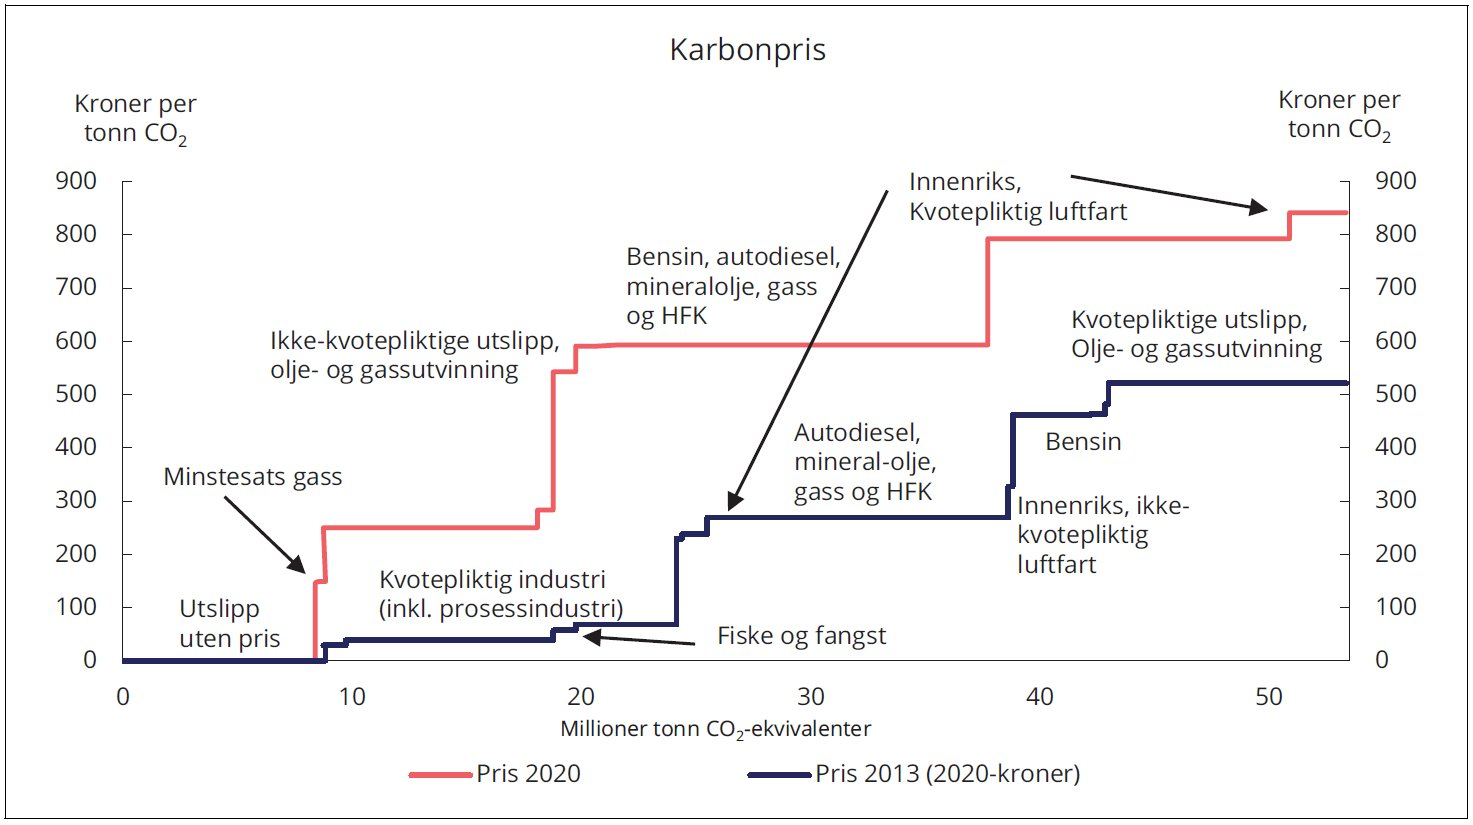
\includegraphics{fig/Norsk_Karbonpris_SM14_2021.jpeg}
\caption{St.meld. 14 (2020-2021)}
\end{figure}

\hypertarget{carbon-offsets}{%
\chapter{Carbon Offsets}\label{carbon-offsets}}

Carbon offset schemes allow individuals and companies to invest in environmental projects around the world in order to balance out their own carbon footprints. The projects are usually based in developing countries and most commonly are designed to reduce future emissions. This might involve rolling out clean energy technologies or purchasing and ripping up carbon credits from an emissions trading scheme. Other schemes work by soaking up CO2 directly from the air through the planting of trees.

\begin{itemize}
\tightlist
\item
  Selling Indulgencies*
  George Monbiot famously compared carbon offsets with the ancient Catholic church's practice of selling indulgences: absolution from sins and reduced time in purgatory in return for financial donations to the church.
  Just as indulgences allowed the rich to feel better about sinful behaviour without actually changing their ways, carbon offsets allow us to buy complacency, political apathy and self-satisfaction.
\end{itemize}

\emph{Additionality}
the key issue for anyone who does want to offset is whether the scheme you're funding actually achieves the carbon savings promised. This boils down not just to the effectiveness of the project at soaking up CO2 or avoiding future emissions. Effectiveness is important but not enough. You also need to be sure that the carbon savings are additional to any savings which might have happened anyway.
The problem is that it's almost impossible to prove additionality with absolute certainly, as no one can be sure what will happen in the future, or what would have happened if the project had never existed.

Partly because of the difficulty of ensuring additionality, many offset providers guarantee their emissions savings. This way, if the emissions savings don't come through or they turn out to be ``non-additional'', the provider promises to make up the loss via another project.

As the offset market grows, some offset companies have enough capital to invest in projects speculatively: they fund an offset project and then sell the carbon savings once the cuts have actually been made. This avoids the difficulty of predicting the future -- and also avoids the claim that a carbon cut made some years in the future is worth less than a cut made now.

These kinds of guarantees and policies provide some reassurances, but do they mean anything in the real world? Without actually visiting the offset projects ourselves, how can individuals be sure that the projects are functioning as they should?

Even if offset projects do work as advertised, some environmentalists argue that they're still a bad idea. If we're to tackle climate change, they argue, the projects being rolled out by offset companies should be happening anyway, funded by governments around the world, while companies and individuals reduce their carbon footprints directly. Only in this way -- by doing everything possible to make reductions everywhere, rather than polluting in one place and offsetting in another -- does the world have a good chance of avoiding runaway climate change, such critics claim.

\emph{Market Standards}
To try and answer these questions, the voluntary offset market has developed various standards, which are a bit like the certification systems used for fairly traded or organic food. These include the Voluntary Gold Standard (VGS) and the Voluntary Carbon Standard (VCS).
Offsets with these standards offer extra credibility, but that still doesn't make them watertight. Heather Rogers, author of Green Gone Wrong, visited a number of offset schemes in India and found all kinds of irregularities.

\emph{Offset Price}
Many people are confused by the low prices of carbon offsets. If it's so bad for the environment to fly, can a few pounds really be enough to counteract the impact? The answer is that, at present, there are all kinds of ways to reduce emissions very inexpensively. After all, a single low-energy lightbulb, available for just £1 or so, can over the space of six years save 250kg of CO2 -- equivalent to a short flight. That's not to say that offsetting is necessarily valid, or that plugging in a low-energy lightbulb makes up for flying. The point is simply that the world is full of inexpensive ways to reduce emissions. In theory, if enough people started offsetting, or if governments started acting seriously to tackle global warming, then the price of offsets would gradually rise, as the low-hanging fruit of emissions savings -- the easiest and cheapest ``quick wins'' -- would get used up.

Another frequent point of confusion about the cost of offsetting is that different offset companies quote different prices for offsetting the same activity. There are two reasons for this. First, there are various ways of estimating the precise impact on climate change of certain types of activity -- including flying, which affects global temperature in various different ways. Second, different types of offset project will inevitably have different costs -- especially given that projects may be chosen not just for the CO2 impacts but for their broader social benefits.

\href{https://www.theguardian.com/environment/2011/sep/16/carbon-offset-projects-carbon-emissions\#:~:text=Carbon\%20offset\%20schemes\%20allow\%20individuals,designed\%20to\%20reduce\%20future\%20emissions.}{Duncan Clark (Guardian 2011): Complete Guide to Carbon Offsetting}

\hypertarget{market-upscaling}{%
\section{Market Upscaling}\label{market-upscaling}}

Carney presented plans at the virtual Davos meeting of global business and political leaders on Wednesday evening for vast increases in the number of carbon offsets sold, aiming to expand the market from about \$300m at present to between \$50bn and \$100bn a year.

He told the conference that he ``categorically rejected'' criticism that offsets were greenwash. Companies buying offsets in the market would be subject to scrutiny, and must have clear plans to reach net zero, ``not something written on the back of a napkin'', he said, but would need offsets to fulfil their plans.

``This is bringing those companies into a formal system,'' he said. ``This is about maximising the use of a very limited {[}global{]} carbon budget. This is complementary {[}to companies taking action to reduce their own emissions{]} and is one piece of the puzzle. We do need this market.''

The leaders of two UK environmental charities have written to Mark Carney, the UN climate envoy and former governor of the Bank of England, to raise concerns over the blueprint for carbon offsetting that could result in billions of new carbon credits being sold around the world.

Campaigners say system risks becoming greenwashing exercise unless loopholes closed.

The markets are used as a cover by companies that wish to give the appearance of working towards net zero emissions but prefer buying cheap credits to the more difficult task of cutting their emissio

This initiative risks setting a terrible example ahead of the critical carbon market negotiations at the global climate summit in Glasgow later this year. {[}It{]} seems to have ignored past failures of offsetting schemes to guarantee emission cuts. At the same time, it assumes that the natural world has unlimited potential to absorb climate-wrecking emissions. It fails to acknowledge that the most important thing companies must do is to reduce their own emissions and use of fossil fuels.

Carney's scheme will serve as a giant get-out-of-jail-free card for polluting companies.

There is a danger that it becomes a large international greenwashing exercise, creating a market with low standards but high PR value,

\href{https://www.theguardian.com/environment/2021/jan/27/green-groups-raise-concerns-over-carney-carbon-credits-plan}{Guardian on Carney Offsets}

\begin{quote}
If you scale a bad thing, it doesn't matter how big you make it, it's still bad.
\end{quote}

As Mark Carney presented the world's top political and business leaders with a blueprint to scale up the voluntary carbon market on Wednesday, campaigners warned key criteria to improve environmental integrity were missing.

With carbon neutrality pledges becoming the benchmark for climate ambition, businesses around the world are looking to offset the emissions they cannot cut and for cheaper ways to meet their climate goals.

Its report identified ways to bring coherence to what is currently a fragmented market. But it said little on how to ensure projects financed through the market deliver genuinely additional emissions reductions.

An open letter to Carney signed by 47 researchers, academics and campaigners ahead of the launch accused the initiative of trying to ``minimise the cost of compliance for private corporations'' at the cost of environmental integrity.

An independent process driven by civil society should define what constitute a quality offset to avoid the private sector self-regulating.

Sequestrating carbon in ecosystems should not replace real emissions cuts.
We need to sequester past emissions that are already in the atmosphere whereas offsetting by definition is about future emissions. The whole point of an offset is that an entity keeps emitting. There is a striking lack of binding and credible measures to actually prioritise emissions reductions.

The biodiversity co-benefits that result from the voluntary carbon market are ``a strong assumption'' with no evidence.

It's important not to forget the huge flows of finance currently facilitating the drivers of biodiversity loss - warning against the market being perceived as an adequate substitute to conservation.

\href{https://www.climatechangenews.com/2021/01/27/carneys-carbon-offset-taskforce-ducks-environmental-integrity-questions/}{ClimateChangeNews}

\emph{Memo TSVCM Report}

Chaired by Bill Winters, group chief executive of Standard Chartered, and sponsored by the Institute of International Finance (IIF), the taskforce includes some of the world's most polluting companies: airline easyJet, plane manufacturer Boeing, oil giants BP, Shell and Total, and steel producer Tata Steel. No green groups are represented among its members.

The need for climate action, and tools to
mobilize finance for the low-carbon and
resilient transition, grows more urgent by the
day. To achieve the Paris goals to limit global
warming to 1.5 degrees Celsius, the global
community needs to reach net-zero emissions
by no later than 2050. This will require a
whole-economy transition---every company,
every bank, every insurer and investor
will have to adjust their business models,
develop credible plans for the transition, and
implement them.

Many companies, especially in hard-to-
abate sectors, will need to offset emissions
as they achieve their decarbonization goals,
creating a surge in demand for credible
offsets.

To facilitate this global
decarbonization there is a need for a large,
transparent, verifiable and robust voluntary
carbon market, one that promotes genuine
action of high environmental integrity.

Along with the carbon avoided, reduced, or
removed, the scaling up of markets has the
further potential to help support financial
flows to the Global South, as activities and
projects in these countries can provide a cost-
effective source of these carbon-emission
reductions. Voluntary carbon markets can
also play a critical role in scaling down cost
curves for emerging climate technologies,
bringing these technologies to market earlier,
and allowing them to be used in direct
decarbonization efforts.

The Taskforce has found
six key areas where efforts are required
to achieve a large, transparent, verifiable,
and robust voluntary carbon market;
these themes are establishing core carbon
principles, core carbon reference contracts,
infrastructure, offset legitimacy, market
integrity, and demand signaling.

!! Direct
emissions reductions by corporates must
be the priority, with appropriate offsetting
playing an important complementary role
to accelerate climate